%%%%%%%%%%%%%%%%%%%%%%%%%%%%%%%%%%%%%%%%%%%%%%%%%%%%%%%%%%%%
%%% LaPreprint: PREPRINT TEMPLATE
%%%%%%%%%%%%%%%%%%%%%%%%%%%%%%%%%%%%%%%%%%%%%%%%%%%%%%%%%%%%

% Here I could talk about what one should do in this document.
% Instead I'll refer you to the explore on your own and check the Github Repo. :-)
% Line spacing is 1.2 by default (can't be smaller).

%%%%%%%%%%%%%%%%%%%%%%%%%%%%%%%%%%%%%%%%%%%%%%%%%%%%%%%%%%%%
%%% PREAMBLE
%%%%%%%%%%%%%%%%%%%%%%%%%%%%%%%%%%%%%%%%%%%%%%%%%%%%%%%%%%%%

% Declare document class
\documentclass[9pt,biorxiv,doublespacing,lineno,endfloat]{lapreprint}
% Choose between "biorxiv", "medrxiv", "arxiv" and "chemrxiv". Otherwise defaults "Preprint".
% Choose between "blue" and "red" colour scheme. Defaults to "blue".
% Use the "onehalfspacing" option for 1.5 line spacing.
% Use the "doublespacing" option for 2.0 line spacing.
% Use the "lineno" option for line numbers.
% Use the "endfloat" option to place floats after the bibliography.

% Import packages
% \usepackage{lipsum}     % Required to insert dummy text
\usepackage[version=4]{mhchem} % For chemical notation
\usepackage{siunitx}    % For SI units
\usepackage{pdflscape}  % For putting pages in landscape mode
\usepackage{rotating}   % For rotating specific elements
\usepackage{textgreek}  % Greek symbols
\usepackage{gensymb}    % Symbols
\usepackage[misc]{ifsym} % For the \Letter symbol
\usepackage{orcidlink}  % For the \orcidlink
\usepackage{listings}   % For inserting code chunks
\usepackage{colortbl}   % For Knitr table colouring
\usepackage{tabularx}   % For making Knitr tables compatible
\usepackage{longtable}  % For multi-page tables
\usepackage{subcaption}
\usepackage{cleveref} % For fig, table and equation numbering
\usepackage{multirow}
\usepackage{snotez}     % For sidenote environments. enotez for endnotes
\usepackage{csquotes}   % For language-based quote rules (helps BiBLaTeX)

\providecommand{\tightlist}{% Command for list
\setlength{\itemsep}{0pt}\setlength{\parskip}{0pt}}

%% Make sure that the picture stay on the page
\makeatletter
\def\maxwidth{\ifdim\Gin@nat@width>\linewidth\linewidth\else\Gin@nat@width\fi}
\def\maxheight{\ifdim\Gin@nat@height>\textheight\textheight\else\Gin@nat@height\fi}
\makeatother
% Scale images if necessary, so that they will not overflow the page
% margins by default, and it is still possible to overwrite the defaults
% using explicit options in \includegraphics[width, height, ...]{}
\setkeys{Gin}{width=\maxwidth,height=\maxheight,keepaspectratio}

%% pandoc-tablenos: required package
\usepackage{caption}

%% pandoc-tablenos: environment to disable table caption prefixes
\makeatletter
\newcounter{tableno}
\newenvironment{tablenos:no-prefix-table-caption}{
  \caption@ifcompatibility{}{
    \let\oldthetable\thetable
    \let\oldtheHtable\theHtable
    \renewcommand{\thetable}{tableno:\thetableno}
    \renewcommand{\theHtable}{tableno:\thetableno}
    \stepcounter{tableno}
    \captionsetup{labelformat=empty}
  }
}{
  \caption@ifcompatibility{}{
    \captionsetup{labelformat=default}
    \let\thetable\oldthetable
    \let\theHtable\oldtheHtable
    \addtocounter{table}{-1}
  }
}
\makeatother

% Make declarations
\DeclareSIUnit\Molar{M}

% Please note that these options may affect formatting. 

%%%%%%%%%%%%%%%%%%%%%%%%%%%%%%%%%%%%%%%%%%%%%%%%%%%%%%%%%%%%
%%% BIBLIOGRAPHY
%%%%%%%%%%%%%%%%%%%%%%%%%%%%%%%%%%%%%%%%%%%%%%%%%%%%%%%%%%%%
% \usepackage[			% use biblatex for bibliography
% 	backend=biber,      % use biber or bibtex backend
%     style=authoryear,   % choose style
% 	natbib=true,		% allow natbib commands
% 	hyperref=true,	    % activate hyperref support
% 	alldates=year,      % only show year (not month)
% ]{biblatex}

% Update to your bibliography file
% \addbibresource{src/bibliography.bib}

% For Pandoc citeproc module support
\newlength{\cslhangindent}
\setlength{\cslhangindent}{1.5em}
\newlength{\csllabelwidth}
\setlength{\csllabelwidth}{3em}
\newlength{\cslentryspacingunit} % times entry-spacing
\setlength{\cslentryspacingunit}{\parskip}
\newenvironment{CSLReferences}[2] % #1 hanging-ident, #2 entry spacing
 {% don't indent paragraphs
  \setlength{\parindent}{0pt}
  % turn on hanging indent if param 1 is 1
  \ifodd #1
  \let\oldpar\par
  \def\par{\hangindent=\cslhangindent\oldpar}
  \fi
  % set entry spacing
  \setlength{\parskip}{#2\cslentryspacingunit}
 }%
 {}
\usepackage{calc}
\newcommand{\CSLBlock}[1]{#1\hfill\break}
\newcommand{\CSLLeftMargin}[1]{\parbox[t]{\csllabelwidth}{#1}}
\newcommand{\CSLRightInline}[1]{\parbox[t]{\linewidth - \csllabelwidth}{#1}\break}
\newcommand{\CSLIndent}[1]{\hspace{\cslhangindent}#1}

%%%%%%%%%%%%%%%%%%%%%%%%%%%%%%%%%%%%%%%%%%%%%%%%%%%%%%%%%%%%
%%% ARTICLE SETUP
%%%%%%%%%%%%%%%%%%%%%%%%%%%%%%%%%%%%%%%%%%%%%%%%%%%%%%%%%%%%

% Paper title
\title{Essential ingredients in Joint Species Distribution Models: how
to optimise inference and prediction in species rich communities?}

% Authors - you can use \orcidlink{} and \authfn{} - see contribution note

% You need to have white spaces around the \orcidlink{} command
% otherwise, LaTeX will raise errors
\author[ \orcidlink{0000-0001-6217-5891} 1\Letter]{Clément Violet}
\author[ \orcidlink{0000-0002-5692-7660} 1]{Aurélien Boyé}
\author[ \orcidlink{0000-0002-1170-5343} 1]{Mathieu Chevalier}
\author[ \orcidlink{0000-0002-4158-7560} 2]{Olivier Gauthier}
\author[ \orcidlink{0000-0002-3107-6740} 3]{Jacques Grall}
\author[ \orcidlink{0000-0002-8152-4273} 1]{Martin P. Marzloff}

% Affiliations
\affil[1]{IFREMER, Centre de Bretagne, DYNECO LEBCO, Plouzané, France}
\affil[2]{Laboratoire des Sciences de l'Environnement Marin (LEMAR) UMR
6539 CNRS UBO IRD IFREMER, Institut Universitaire Européen de la Mer,
Université de Bretagne Occidentale, Plouzané, France}
\affil[3]{Observatoire des Sciences de l'Univers, UMS 3113, Institut
Universitaire Européen de la Mer, Plouzané, France}

% Other metadata. Feel free to add your own
\metadata[]{\Letter\hspace{.5ex} For correspondence}{\href{mailto:}{clement.violet@ifremer.fr}}
\metadata[]{Present address}{IFREMER, Centre de Bretagne, DYNECO LEBCO,
Plouzané 29280, France.}
\metadata[]{Keywords}{Community assembly, Explanatory power, Joint
Species Distribution Model, jSDM, Model Performances, Predictive
power, Species Distribution Model}
\metadata[]{Competing interests}{The authors declare no competing
interests.}
% \metadata[\authfn{1}\authfn{2}\authfn{3}]{}{Here's a few symbols to denote contribution specifics, e.g. authors who contributed equally to the work.}

% Surname of the lead author(s) for the running footer
\leadauthor{Violet}
\shorttitle{Essential ingredients in Joint Species Distribution Models}

%%%%%%%%%%%%%%%%%%%%%%%%%%%%%%%%%%%%%%%%%%%%%%%%%%%%%%%%%%%%
%%% ARTICLE START
%%%%%%%%%%%%%%%%%%%%%%%%%%%%%%%%%%%%%%%%%%%%%%%%%%%%%%%%%%%%

\begin{document}
\maketitle

\begin{abstract}

\begin{enumerate}
\def\labelenumi{\arabic{enumi}.}
\item
  Joint Species Distribution Models (jSDM) can be powerful and versatile
  tools to explain and predict the spatio-temporal variability of
  species communities, which are critical research questions at the
  forefront of modern ecology. For instance, jSDM can include phylogeny
  or functional traits and can account for residual co-occurrences
  patterns between species to capture the processes shaping communities
  and their evolution in a changing world. However, the effects of
  including heterogeneous information sources in jSDMs has not been
  formally assessed while it raises a number of questions related to
  their influence on model interpretability and performance.
\item
  Here, we investigated the effects on jSDM of including additional
  information, either species-specific information such as phylogeny
  and/or traits, or community monitoring data related to accompanying
  species (i.e sampled at the same time as the target species
  community). Based on a typical regional case study, we focus on
  space-time variability in community structure to specifically assess
  how alternative model formulations (that includes, or not, additional
  information) affect jSDM interpretability, explanatory and predictive
  power.
\item
  Our results show that jSDM ability to predict variability in targeted
  species assemblage can be improved by including monitoring data
  related to accompanying species in the model. Moreover, addition of
  accompanying species clarifies species-environment relationships by
  filtering out the weak/spurious correlation inferred in the baseline
  model. While addition of species-specific information for the target
  species community (e.g.~traits) does not improve model predictive
  performance, it nevertheless provides some insights on how species of
  interest respond to environmental gradients, and hence improves model
  interpretability.
\item
  This work provides important new guidelines for ecological researchers
  in terms of appropriate strategies to adopt for jSDM fitting as a
  function of their modelling objective(s) and/or research questions. If
  the primary goal lies in understanding observed space-time variability
  in a given species community, then adding species-specific phylogeny
  or traits appears as an appropriate strategy. Inclusion of
  accompanying species is however a better strategy if the primary
  research aim is to predict how the observed species assemblage of
  interest responds to environmental changes or to alternative
  scenarios.
\end{enumerate}
\end{abstract}

\hypertarget{introduction}{%
\section{Introduction}\label{introduction}}

Community ecology aims at explaining and predicting spatio-temporal
variability in species diversity
(\protect\hyperlink{ref-Whittaker_2001}{Whittaker \emph{et al.} 2001})
and coexistence (\protect\hyperlink{ref-Chesson_2000}{Chesson 2000}).
Understanding the processes that determine species distribution around
the planet is a prerequisite to characterise and predict community
structure and associated ecological dynamics, which is critical to
mitigate the effects of global change on biodiversity and prevent the
sixth mass extinction (\protect\hyperlink{ref-ipbes_2019}{IPBES 2019}).
Currently, the major challenges faced by ecologists include describing,
explaining, and predicting changes in communities
(\protect\hyperlink{ref-Tredennick_2021}{Tredennick \emph{et al.} 2021})
in order to inform effective management or restoration measures in a
rapidly changing world (\protect\hyperlink{ref-Houlahan_2017}{Houlahan
\emph{et al.} 2017}; \protect\hyperlink{ref-Dietze_2018}{Dietze \emph{et
al.} 2018}; \protect\hyperlink{ref-Brudvig_2022}{Brudvig \& Catano
2022}). Joint Species Distribution Models (jSDM) are particularly
well-suited tools to address these challenges, whether to characterise
the processes that shape observed communities
(\protect\hyperlink{ref-Ovaskainen_2017a}{Ovaskainen \emph{et al.}
2017b}), or to predict how communities will evolve in the future
(\protect\hyperlink{ref-Norberg_2019}{Norberg \emph{et al.} 2019}).

jSDMs are multivariate (i.e.~multi-species) extensions of Species
Distribution Models (SDMs), which have been broadly applied over the
past decades - across all terrestrial and marine realms - to understand
and predict both species occurrences
(\protect\hyperlink{ref-Elith_2006}{Elith \emph{et al.} 2006} ;
\protect\hyperlink{ref-Norberg_2019}{Norberg \emph{et al.} 2019}) and
species abundances (\protect\hyperlink{ref-Howard_2014}{Howard \emph{et
al.} 2014} ; \protect\hyperlink{ref-Waldock_2022}{Waldock \emph{et al.}
2022}) using a set of covariates (e.g.~climatic variables). One
advantage of jSDM relies on their explanatory power owing to their tight
link with the assembly rule framework
(\protect\hyperlink{ref-Ovaskainen_2017a}{Ovaskainen \emph{et al.}
2017b}). In particular, relative to single-species SDMs that only
consider the abiotic niche of species (i.e.~the Grinellian niche), jSDM
can theoretically also account for interspecific interactions (i.e.~the
Eltonian niche).

Indeed, in jSDMs, the variability in community composition not explained
by covariates is captured by a residual covariance matrix representing
species co-occurence patterns potentially representing biotic
interactions (\protect\hyperlink{ref-Ovaskainen_2017a}{Ovaskainen
\emph{et al.} 2017b}). This feature is highly attractive to ecologists
because it provides a way to disentangle the relative influence of
abiotic and biotic processes on biodiversity patterns
(\protect\hyperlink{ref-Godsoe_2017}{Godsoe \emph{et al.} 2017}) while
also improving model's predictive power
(\protect\hyperlink{ref-Giannini_2013}{Giannini \emph{et al.} 2013};
\protect\hyperlink{ref-Staniczenko_2017}{Staniczenko \emph{et al.}
2017}). However, in practice, inferring and interpreting residual
co-occurence patterns using jSDMs remains challenging for several
reasons (\protect\hyperlink{ref-Blanchet_2020}{Blanchet \emph{et al.}
2020} ; \protect\hyperlink{ref-Holt_2020}{Holt 2020}).

First, while jSDMs have been applied to a large number of species
presence/absence datasets (\protect\hyperlink{ref-Norberg_2019}{Norberg
\emph{et al.} 2019} ; \protect\hyperlink{ref-Wilkinson_2019}{Wilkinson
\emph{et al.} 2019} ; \protect\hyperlink{ref-Wilkinson_2020}{Wilkinson
\emph{et al.} 2020}), simulation studies showed that co-occurence
networks inferred from such data does not necessarily provide evidence
for species interactions (\protect\hyperlink{ref-Blanchet_2020}{Blanchet
\emph{et al.} 2020} ; \protect\hyperlink{ref-Dormann_2018}{Dormann
\emph{et al.} 2018} ; \protect\hyperlink{ref-Sander_2017}{Sander
\emph{et al.} 2017}) and only inform about spatial and temporal
associations between species (\protect\hyperlink{ref-Keil_2021}{Keil
\emph{et al.} 2021}). Some authors speculated that jSDMs applied to
abundance data - instead of presence/absence data - are likely to
provide a better proxy for biotic interactions
(\protect\hyperlink{ref-Blanchet_2020}{Blanchet \emph{et al.} 2020} ;
\protect\hyperlink{ref-Momal_2020}{Momal \emph{et al.} 2020}).
Accordingly, jSDM have progressively been extended and applied to
abundance data (\protect\hyperlink{ref-Chiquet_2021}{Chiquet \emph{et
al.} 2021} ; \protect\hyperlink{ref-Hui_2016}{Hui 2016} ;
\protect\hyperlink{ref-Ovaskainen_2017a}{Ovaskainen \emph{et al.} 2017b}
; \protect\hyperlink{ref-Popovic_2022}{Popovic \emph{et al.} 2022}).
Yet, specific challenges related to modelling abundance data have only
been recently explored in the context of species distribution modelling
(\protect\hyperlink{ref-Waldock_2022}{Waldock \emph{et al.} 2022}). To
date, the predictive and the explanatory power of jSDM fitted to
abundance data remains largely untested compared to presence/absence
data (\protect\hyperlink{ref-Norberg_2019}{Norberg \emph{et al.} 2019} ;
\protect\hyperlink{ref-Wilkinson_2020}{Wilkinson \emph{et al.} 2020}).

Second, regardless of the type of data considered (i.e.~presence/absence
or abundance), several factors may limit or affect the interpretability
and predictive ability of jSDM. For instance, co-occurence patterns
estimated in jSDM are affected by unaccounted environmental variables
implying that jSDMs cannot fully separate the environmental and the
biotic niche of species (\protect\hyperlink{ref-Blanchet_2020}{Blanchet
\emph{et al.} 2020} ; \protect\hyperlink{ref-Poggiato_2021}{Poggiato
\emph{et al.} 2021}). Beyond missing environmental predictors, one
prerequisite for improving biotic inference and thus jSDMs' predictions
is to take into account other actors (i.e.~species) that could have an
influence on the target community (e.g.~competitors; Levine \emph{et
al.} (\protect\hyperlink{ref-Levine_2017}{2017})). However, because many
ecological studies only focus on particular taxonomic groups
(\protect\hyperlink{ref-Pollock_2014}{Pollock \emph{et al.} 2014} ;
\protect\hyperlink{ref-Hakkila_2018}{Häkkilä \emph{et al.} 2018}), hence
disregarding non-target taxa, co-occurence patterns estimated from jSDMs
are almost always skewed by missing ecological actors
(\protect\hyperlink{ref-Momal_2021}{Momal \emph{et al.} 2021}). How this
bias affects the predictive ability of jSDM remains untested.

Finally, similarly to SDMs, jSDMs can theoretically be extended to
include additional sources of information about modelled species
(\protect\hyperlink{ref-Niku_2019}{Niku \emph{et al.} 2019} ;
\protect\hyperlink{ref-Ovaskainen_2017a}{Ovaskainen \emph{et al.}
2017b}). For instance, accounting for phylogenetic relationships between
species (\protect\hyperlink{ref-Ives_2011}{Ives \& Helmus 2011}) or for
the link between functional traits and environmental responses
(\protect\hyperlink{ref-Pollock_2012}{Pollock \emph{et al.} 2012}) have
been shown to improve both the explanatory and the predictive powers of
SDMs (\protect\hyperlink{ref-Morales-Castilla_2017}{Morales-Castilla
\emph{et al.} 2017} ; \protect\hyperlink{ref-Vesk_2021}{Vesk \emph{et
al.} 2021}), which supports the hypothesis that similar species in terms
of traits and/or recent evolutionary history share similar environmental
preferences. While similar effects related to inclusion of
species-specific information areexpected in jSDMs
(\protect\hyperlink{ref-Ovaskainen_2017a}{Ovaskainen \emph{et al.}
2017b}), the relative influence of additional sources of information on
their interpretability and predictive power remains untested
(\protect\hyperlink{ref-Norberg_2019}{Norberg \emph{et al.} 2019} ;
\protect\hyperlink{ref-Wilkinson_2019}{Wilkinson \emph{et al.} 2019}).

Overall, many practical questions remain concerning the application of
jSDMs to ecological community monitoring data in particular related to
inclusion of additional sources of information within the models. In
this study, we aim to provide a comprehensive assessment of how jSDM
predictive and explanatory powers are affected by different sources of
information. Specifically, by comparing predictions obtained from a
baseline model excluding additional sources of information (i.e.~a
classical jSDM), we tested the effect of (1) including phylogeny alone
and in combination with trait data, (2) incorporating monitoring
information related non-target species and (3) considering abundance
instead of occurrence data. We hypothesised that all these sources of
information should improve jSDM predictive and explanatory powers, but
did not assume \emph{a priori} that a given modelling strategy would
lead to greater improvements in model performances.

\hypertarget{methods-materials}{%
\section{Methods \& Materials}\label{methods-materials}}

We used the HMSC (Hierarchical Modeling of Species Communities)
framework applied to the long-term REBENT coastal monitoring dataset
(\href{https://rebent.ifremer.fr}{rebent.ifremer.fr}). In the following
subsections, we sequentially describe: (1) the HMSC framework;(2) the
data used in this study; (3) data splitting between training and testing
sets to assess the explanatory and predictive powers of models,
respectively; (4) the rationales for the suite of alternative models
considered; and, (5) the performance metrics used to compare models.

\begin{figure}
\hypertarget{fig:workdlow}{%
\centering
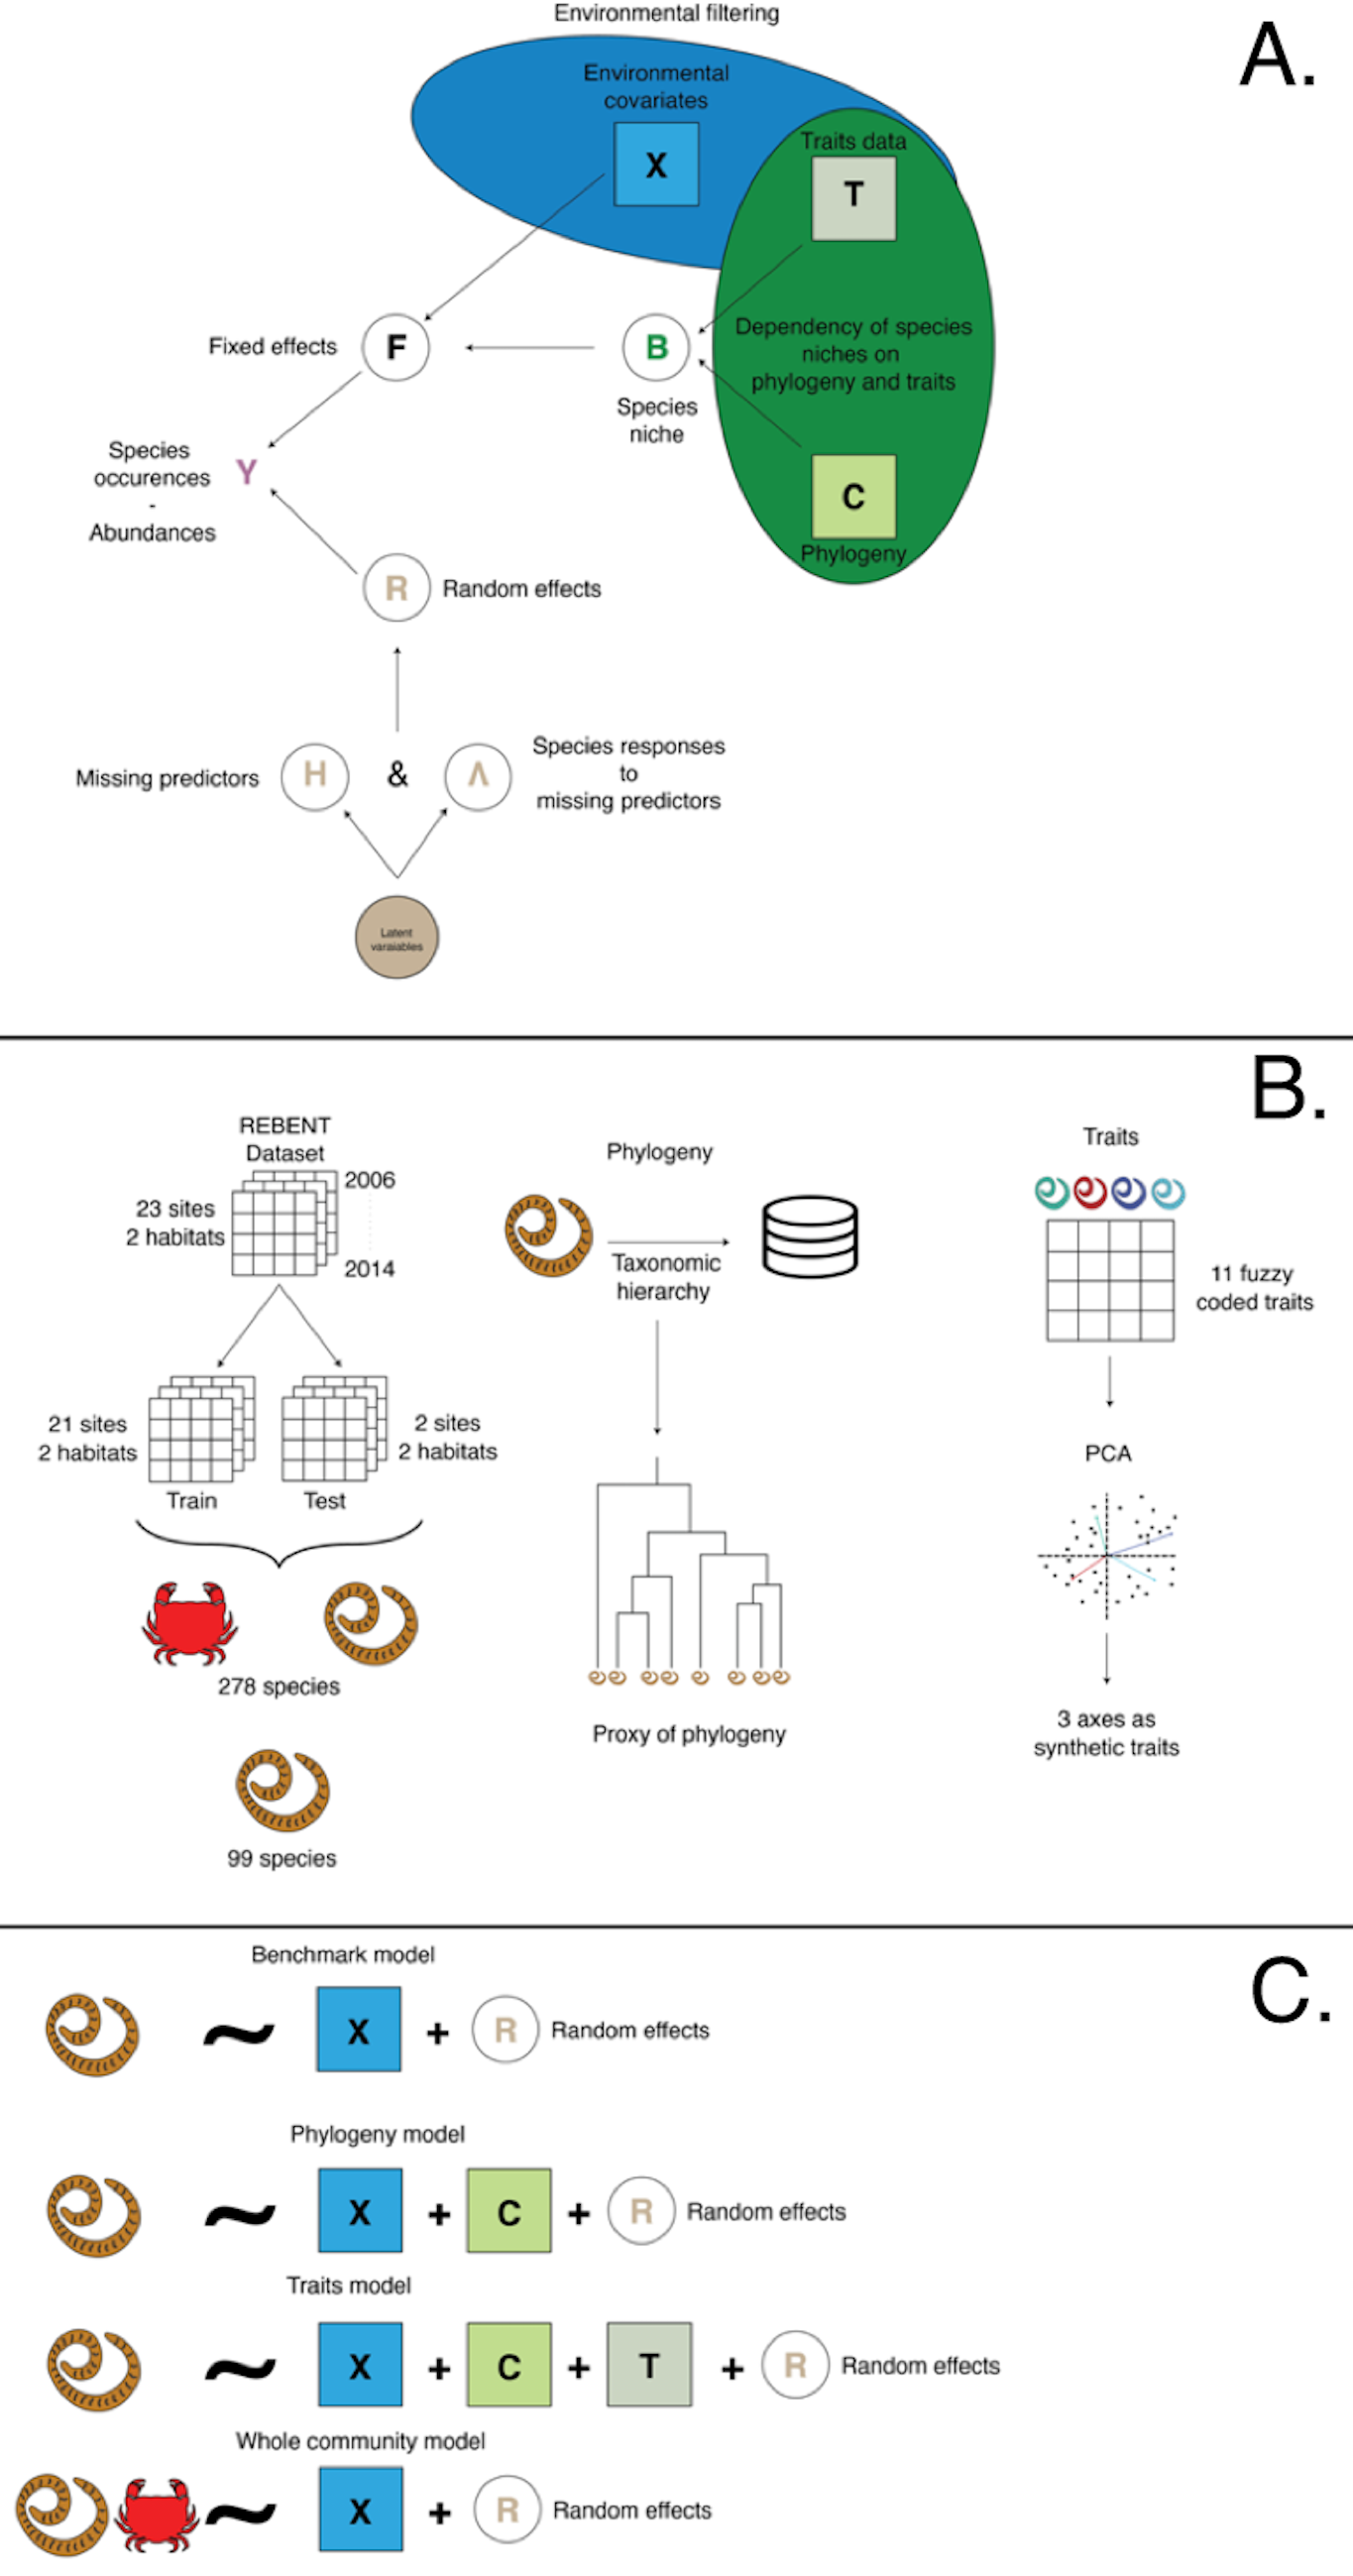
\includegraphics{figures/fig1.png}
\caption{Workflow of the study. A. Hierarchical design of a HMSC model
set-up with environmental variables, phylogeny and traits. B. Data
acquisition workflow. C. Configuration of the differents
models.}\label{fig:workdlow}
}
\end{figure}

\hypertarget{hierarchical-modelling-of-species-community-hmsc}{%
\subsection{Hierarchical Modelling of Species Community
(HMSC)}\label{hierarchical-modelling-of-species-community-hmsc}}

``HMSC is a multivariate hierarchical generalised linear mixed model
adjusted with Bayesian inference rooted in assembly theory''
(\protect\hyperlink{ref-Ovaskainen_2020}{Ovaskainen \& Abrego 2020}). A
HMSC model is composed of two parts: one taking into account fixed
effects and the other taking into account random effects. The fixed part
models the realised niche (i.e., the set of environmental conditions
that is biotically suitable and accessible to the species; Ovaskainen \&
Abrego (\protect\hyperlink{ref-Ovaskainen_2020}{2020})) of each species
(B matrix), where each dimension of the niche is a covariate
(e.g.~temperature) included in the model
(\protect\hyperlink{ref-Ovaskainen_2020}{Ovaskainen \& Abrego 2020}).
Including trait data enables estimating of species-specific expected
niche value by accounting for trait-environment relationships, where
species with similar traits are expected to respond similarly along
environmental gradients
(\protect\hyperlink{ref-Ovaskainen_2017a}{Ovaskainen \emph{et al.}
2017b} ; \protect\hyperlink{ref-Ovaskainen_2020}{Ovaskainen \& Abrego
2020}). It is well-established that phylogenetically-close species tend
to share similar trait values or niches
(\protect\hyperlink{ref-Wiens_2010}{Wiens \emph{et al.} 2010}). Adding
phylogenetic data to a HMSC model already including traits is not
necessarily redundant because it could capture residual ecological
information not included in the available trait data. This can
theoretically enhance estimating of species niches
(\protect\hyperlink{ref-Ovaskainen_2020}{Ovaskainen \& Abrego 2020}).
Inclusion of such additional pieces of information can moreover improve
model fit for rare species by borrowing information on traits- (or
phylogenetic-) environment relationships estimated for common species
that are similar in terms of traits (or phylogenetic; Ovaskainen \&
Abrego (\protect\hyperlink{ref-Ovaskainen_2020}{2020})). This property
is a main advantage of hierarchical models
(\protect\hyperlink{ref-Gelman_2020}{Gelman \emph{et al.} 2020}).

The random part of HMSC relies on latent variables. Specifically, for
each random effect, two matrices of latent variables are estimated
(\protect\hyperlink{ref-Ovaskainen_2017a}{Ovaskainen \emph{et al.}
2017b} ; \protect\hyperlink{ref-Tikhonov_2019b}{Tikhonov \emph{et al.}
2019} ; \protect\hyperlink{ref-Ovaskainen_2020}{Ovaskainen \& Abrego
2020}): the \(H\) matrix (called \emph{site loadings}) contains the
values of missing covariates not included in the model
(\protect\hyperlink{ref-Ovaskainen_2017a}{Ovaskainen \emph{et al.}
2017b} ; \protect\hyperlink{ref-Ovaskainen_2020}{Ovaskainen \& Abrego
2020}); while the \(\Lambda\) matrix (called \emph{species loadings})
corresponds to the response of the species to missing covariates
(\protect\hyperlink{ref-Ovaskainen_2017a}{Ovaskainen \emph{et al.}
2017b} ; \protect\hyperlink{ref-Ovaskainen_2020}{Ovaskainen \& Abrego
2020}). These covariates thus capture residual variance, which can be
due to various factors including missing environmental features or the
effect of biotic interactions
(\protect\hyperlink{ref-Ovaskainen_2017a}{Ovaskainen \emph{et al.}
2017b} ; \protect\hyperlink{ref-Ovaskainen_2017b}{Ovaskainen \emph{et
al.} 2017a} ; \protect\hyperlink{ref-Ovaskainen_2020}{Ovaskainen \&
Abrego 2020}).

\hypertarget{datasets}{%
\subsection{Datasets}\label{datasets}}

\hypertarget{faunistic-data}{%
\subsubsection{Faunistic data}\label{faunistic-data}}

Faunistic data come from the REBENT program
(\href{https://rebent.ifremer.fr}{rebent.ifremer.fr}), which is a
station-based monitoring network initiated following the dramatic oil
spill of the Erika tanker in December 1999 off Brittany's southern
coastline (Western France). The goal of the monitoring network is to
detect, characterise and explain changes in French coastal benthic
ecosystems through space and time. Between 2003 and 2017, this ongoing
program has been monitoring four distinct habitats across 49 sites.
Overall, across a total of 375 sampling units (i.e.~unique combination
of years, sites and habitats), 861,997 individuals belonging to 821
species were collected and identified since the beginning of the program
Here, we focused on benthic communities found in two soft-bottom
habitats: intertidal bare sediments and intertidal seagrass meadows
(\emph{Zostera marina}). These habitats were sampled following the same
protocol across 23 sites along Brittany's coastline (Fig S1). At each
site, sampling consists in collection of 3 sediment cores of 0.03m2 that
are pooled together and considered as a single sampling unit at each
site. For each sampling event, individuals were identified to the lowest
taxonomic level possible (mostly species level). A detailed description
of the sampling methodology is provided in Boyé \emph{et al.}
(\protect\hyperlink{ref-Boye_2017}{2017}).

\hypertarget{functional-traits-and-phylogeny-data}{%
\subsubsection{Functional traits and phylogeny
data}\label{functional-traits-and-phylogeny-data}}

In this study, we collated species-specific information such as
functional traits and phylogeny for inclusion in different models. We
chose to focus on a particular class, the polychaeta. Polychaeta, which
encompasses numerous species that exhibit diverse lifestyles
(\protect\hyperlink{ref-Jumars_2015}{Jumars \emph{et al.} 2015}), are
valuable indicators of the health of benthic habitats
(\protect\hyperlink{ref-Giangrande_2005}{Giangrande \emph{et al.}
2005}). The polychaeta traits data, which was available for the 99
polychaeta species in the training set, includes 11 fuzzy-coded traits
for a total of 41 modalities (\protect\hyperlink{ref-Boye_2019a}{Boyé
\emph{et al.} 2019}). Prior to jSDM fitting, the dimensionality of the
trait matrix was reduced using a fuzzy-PCA with the \emph{fpca} function
from the \emph{ade4} R package
(\protect\hyperlink{ref-Thioulouse_2018}{Thioulouse \emph{et al.}
2018}). The first three axes, which account for 59\% of the total
variance of the trait matrix, were included in the model as synthetic
traits data (Fig S5) . The first axis distinguishes mobile predatory
species from sessile microphages; the second axis differentiates
semelparous species from iteroparous species; and, the third axis
separates burrowers from tube-dwellers (Fig S5).

In complement to the traits information available for the 99 polychaeta
species of interest, we retrieved their taxonomic classification through
the WoRMS database
(\href{https://www.marinespecies.org}{www.marinespecies.org}) and used
this information as a proxy for phylogenetic relationships
(\protect\hyperlink{ref-Ovaskainen_2020}{Ovaskainen \& Abrego 2020} ;
\protect\hyperlink{ref-Ricotta_2012}{Ricotta \emph{et al.} 2012}).
Phylogenetic distances between Polychaeta species were then estimated
using the \emph{ape} R package
(\protect\hyperlink{ref-Paradis_2019}{Paradis \& Schliep 2019}).

\hypertarget{environmental-data}{%
\subsubsection{Environmental data}\label{environmental-data}}

Based on Boyé (\protect\hyperlink{ref-Boye_2019b}{2019}), we selected
seven environmental variables to characterise the ecological niche of
each species within the focal communities. These seven variables
quantify different components of coastal environmental variability
including hydrology (sea water temperature, salinity and current
velocity), sedimentology (mud and organic matter content), granulometry
(Trask index) and local wave exposure (fetch). For each variable, the
first and second degree polynomials have been computed to account for
non-linear responses to the environmental predictors.

\hypertarget{comparison-of-alternative-model-structures}{%
\subsection{Comparison of alternative model
structures}\label{comparison-of-alternative-model-structures}}

The first model (benchmark model abbreviated as ``Bench'') only relies
on polychaeta community data and environmental covariates. The second
model (phylogenetic model abbreviated as ``Ph'') adds phylogenetic data
to the Bench model, which implies that rare species can thus benefit
from phylogenetic-environment relationships estimated for closely
related species (\protect\hyperlink{ref-Ives_2011}{Ives \& Helmus
2011}). The third model (traits-phylogeny model abbreviated as ``TrPh'')
adds traits data to the Ph model, which means that rare species can
benefit from traits-environment relationships estimated for species
presenting similar functional traits (whereas phylogeny can capture
ecological similarities between species, which are not captured by trait
similarity; (\protect\hyperlink{ref-Pollock_2012}{Pollock \emph{et al.}
2012})). Finally, the fourth model (whole community model abbreviated as
``Whc''), adds information about the whole community
(i.e.~non-polychaeta species that represents 278 taxa) to the Bench
model (only 99 polychaeta). This model does not include trait or
phylogenetic data for the sake of computation time. Each of these four
models were fitted twice, either using occurrence or abundance data. All
models include the same random effects: a temporal random effect to
account for variability across years, a spatial random effect to account
for variability across sites and another spatial random effect to
account for variability across habitats (bare vs seagrass).

\hypertarget{model-fitting-and-performance}{%
\subsection{Model fitting and
performance}\label{model-fitting-and-performance}}

\hypertarget{model-fitting-using-markov-chain-monte-carlo}{%
\subsubsection{Model fitting using Markov Chain Monte
Carlo}\label{model-fitting-using-markov-chain-monte-carlo}}

HMSC uses a Bayesian framework for model fitting where the posterior
distribution is sampled using a MCMC algorithm. For each model we ran 15
chains, each with 30,000 iterations. The first 10,000 iterations were
discarded as burn-in while the remaining were thinned every 20
iterations yielding 1,000 posterior samples per chain. Hence, in total,
15,000 posterior samples were recorded for each parameter. Model
convergence for each model parameter was assessed using the potential
scale reduction factor (\protect\hyperlink{ref-Gelman_1992}{Gelman \&
Rubin 1992}).

\hypertarget{assessing-model-performance-and-interpretability}{%
\subsubsection{Assessing model performance and
interpretability}\label{assessing-model-performance-and-interpretability}}

In order to independently assess models' predictive performance, the
REBENT dataset was split into a train and a test dataset. The
\emph{training dataset} includes 180 sampling units defined as unique
combinations of years (varies between 6 and 9 depending on sites), sites
(21) and habitats (2). From this dataset, we removed the species that
occurred less than 4 times across the 180 observational units to avoid
convergence issues and poor model inference, leading to the removal of
241 species. The remaining 278 species encompassed the 99 polychaeta
species that made up the target community and the 142 accompanying
species that were included in the \emph{Whc} model. The \emph{test
dataset} was composed of 35 sampling units resulting from surveys
conducted across two specific sites (9 years for both), which included
the two habitats. To investigate jSDM's performance, models were
evaluated using a set of complementary metrics to evaluate both their
explanatory (predictions compared to observations of the train dataset)
and predictive (predictions compared to observations of the test
dataset) powers (\protect\hyperlink{ref-Wilkinson_2020}{Wilkinson
\emph{et al.} 2020}). The performance of all models was assessed
globally but also separately for each species using AUC for
occurrence-based models and root mean squared errors (RMSE) for
abundance-based models. We investigated whether models including
additional sources of information had a higher performance than the
\emph{Bench} model using Dunn's multiple comparison test
(\protect\hyperlink{ref-Dunn_1964}{Dunn 1964}). For the model that
demonstrated the best improvement, we examined whether the improvement
correlated with individual species occurrence or abundance (e.g., is the
improvement higher for abundant species relative to than for rare
species?) using the Kendall rank correlation coefficient.

While the AUC and the RMSE can be used to explore model performance
globally or for each species, these measures provide no information at
the community scale. Hence, we also explored qualitatively the
differences between observed and predicted community composition (both
for the train and test datasets) by decomposing the total beta diversity
(using the Sørensen index) into species turnover and nestedness using
the \emph{betapart.temp} function from the betapart R package
(\protect\hyperlink{ref-Baselga_2010}{Baselga 2010} ;
\protect\hyperlink{ref-Baselga_2022}{Baselga \emph{et al.} 2022}). For
abundance-based models, predictions were transformed to presence/absence
before computing beta diversity (i.e.~all predictions with abundance
different than zero were considered as presences). Under this framework,
a model predicting the exact observed community would have a total beta
diversity of zero whereas a model predicting a community completely
different from the one observed would have a total beta diversity of
one. As outlined above, the Baselga's framework allows decomposition
into two components the type of error when predicting community
composition: (1) getting the identity of the species wrong (turnover) or
(2) predicting the right species but omitting some (nestedness). In the
first case, the model will correctly predict specific richness, while in
the other case the model will be more conservative in predicting the
correct species but present a bias in species richness.

To assess model interpretability, we calculated the proportion of
explained variance attributed either to environmental covariates (fixed
effects) or to random effects. To evaluate the effect of model structure
on estimated species-environment relationships, we classified the shapes
of the response curves inferred from the different models according to
both their direction (decline, null or increase) and their acceleration
(decelerated, constant or accelerated), providing nine different
categories (\protect\hyperlink{ref-Rigal_2020}{Rigal \emph{et al.}
2020}). We then looked for differences between models regarding the
proportion of response curves attributed to each category.

Finally, we checked the extent to which estimated correlation
coefficients differed between the Bench model and the best performing
model while also looking for evidence of inversion of effects using the
following index:

\[\text{Index} = |corr_{\text{best model}} - corr_{\text{benchmark}}| * sign(corr_{\text{best model}} * corr_{\text{benchmark}})\]

\hypertarget{results}{%
\section{Results}\label{results}}

The MCMC convergence and the effective sample size of the different HMSC
models were satisfactory (see Appendix B).

\hypertarget{model-fit-predictive-power}{%
\subsection{Model Fit \& Predictive
power}\label{model-fit-predictive-power}}

\hypertarget{species-level}{%
\subsubsection{Species level}\label{species-level}}

Occurrence-based models presented an excellent explanatory power, with
the AUC being on average greater than 0.9 (Figure S4). Their predictive
power was significantly lower with the AUC being about 0.65 on average
(Figure S4). For abundance-based models, the RMSE computed on the
\emph{training set} ranged from 8.92 to 9.34 on average (Figure S4).
Their predictive power was heterogeneous with the \emph{whole community}
(\emph{WhC}) model (RMSE = 5.83 on average) performing better (Figure
S4) than the three other models (RMSE values ranged from 54.2 to 95.6,
on average).

For the sake of interpretability, all models were compared against
\emph{Bench} model (\cref{fig:fig2}). Model's explanatory power was not
significantly improved for both \emph{TrPh} and \emph{Ph} models and
only slightly increased for the \emph{WhC} models (both occurrence- and
abundance-based). This increase in explanatory power was modest with the
AUC only increasing by 0.0034 ± 0.0114 (mean ± sd) for occurence-based
models and the RMSE only decreasing by 0.035 ± 0.796 (mean ± sd) for
abundance-based models. This improvement mainly concerned the most
common and abundant species, as reflected by the negative correlations
between species-specific RMSE and mean species occurrence (Kendall's τ =
-0.28, p-value \textless{} 1e-5) or mean species abundance (Kendall's τ
= -0.29, p-value \textless{} 1e-4). In terms of predictive power,
performance only significantly increased for the \emph{Whc}
abundance-based model with a decrease in RMSE of 0.27 ± 0.44 (mean ± sd)
relative to the \emph{Bench} model.

\begin{figure}
\hypertarget{fig:fig2}{%
\centering
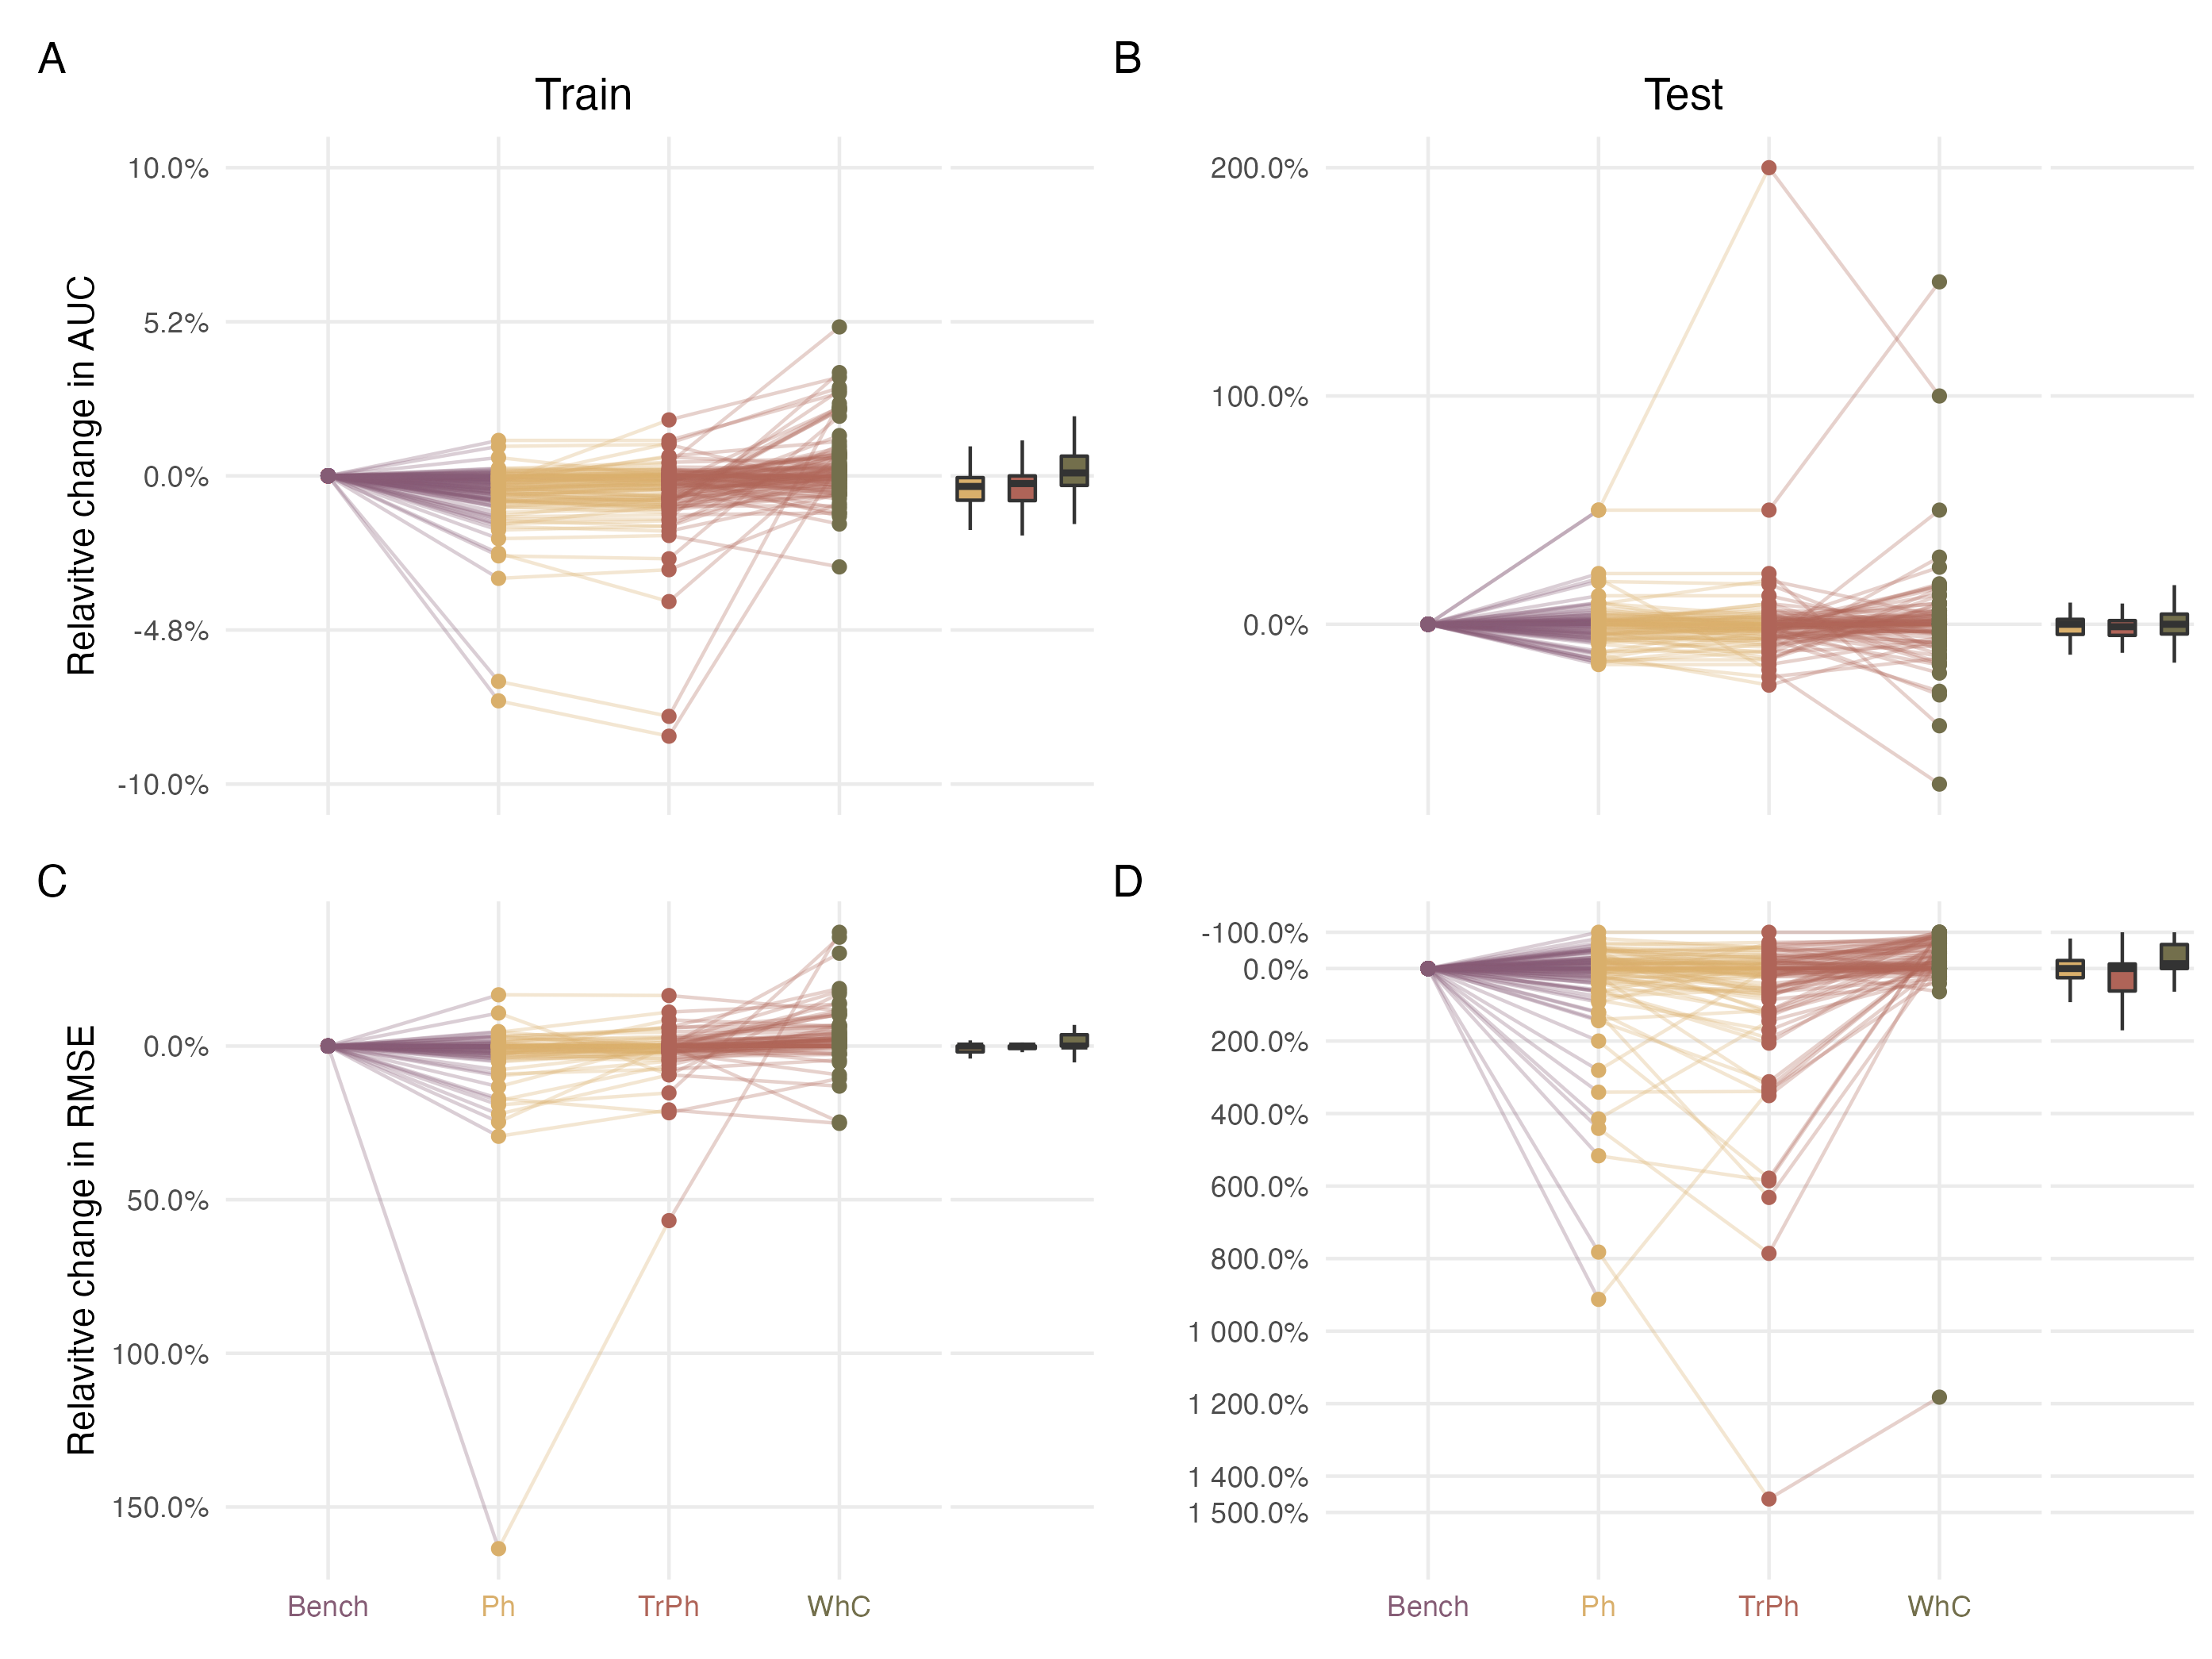
\includegraphics{figures/fig2.png}
\caption{Relative change in explanatory (left column) and predictive
(right column) power of different model architectures with respect to
the benchmark fitted with occurrence (top line) or abundance (bottom
line) data.}\label{fig:fig2}
}
\end{figure}

\hypertarget{community-level}{%
\subsubsection{Community level}\label{community-level}}

On the training set, the median Sørensen dissimilarity ranged from 0.36
to 0.38 across models (both occurrence- and abundance-based), suggesting
that predicted communities are relatively similar to observed
communities (Figure S8 and Figure S9). Errors were equally distributed
between turnover and nestedness. With the test data set, abundance-based
models presented a median Sørensen dissimilarity of 0.65 while
dissimilarity reached 0.72 for occurrence-based models (Figure S8 and
Figure S9). This increased dissimilarity relative to predictions made on
the training dataset is a direct consequence of the degradation of the
predictive power of the various models at the species scale (see above).
Note that the \emph{Whc} model makes more nestedness errors than the
others, suggesting that this model is more conservative in terms of
community composition (Figure S8 and Figure S9).

\hypertarget{variance-partitioning}{%
\subsection{Variance partitioning}\label{variance-partitioning}}

The amount of variance explained by each model can be decomposed between
environmental covariates and random effects. For all models, the
environmental variables account for most (\textgreater{} 75 \% ± 18, on
average) of the explained variance (Figure S7). However, compared to the
\emph{Bench} model, a larger part of variance is explained by the random
effect in the \emph{WhC} model (Figure S7).For abundance-based models,
the median of the relative change in variance explained by random
effects relative to the \emph{Bench} model increased by 0.086 for the
\emph{Ph} model, 0.199 for the \emph{TrPh} model and 0.354 for the
\emph{WhC} model (\cref{fig:fig3}). Similar results were obtained for
occurrence-based models (\cref{fig:fig3}).

\begin{figure}
\hypertarget{fig:fig3}{%
\centering
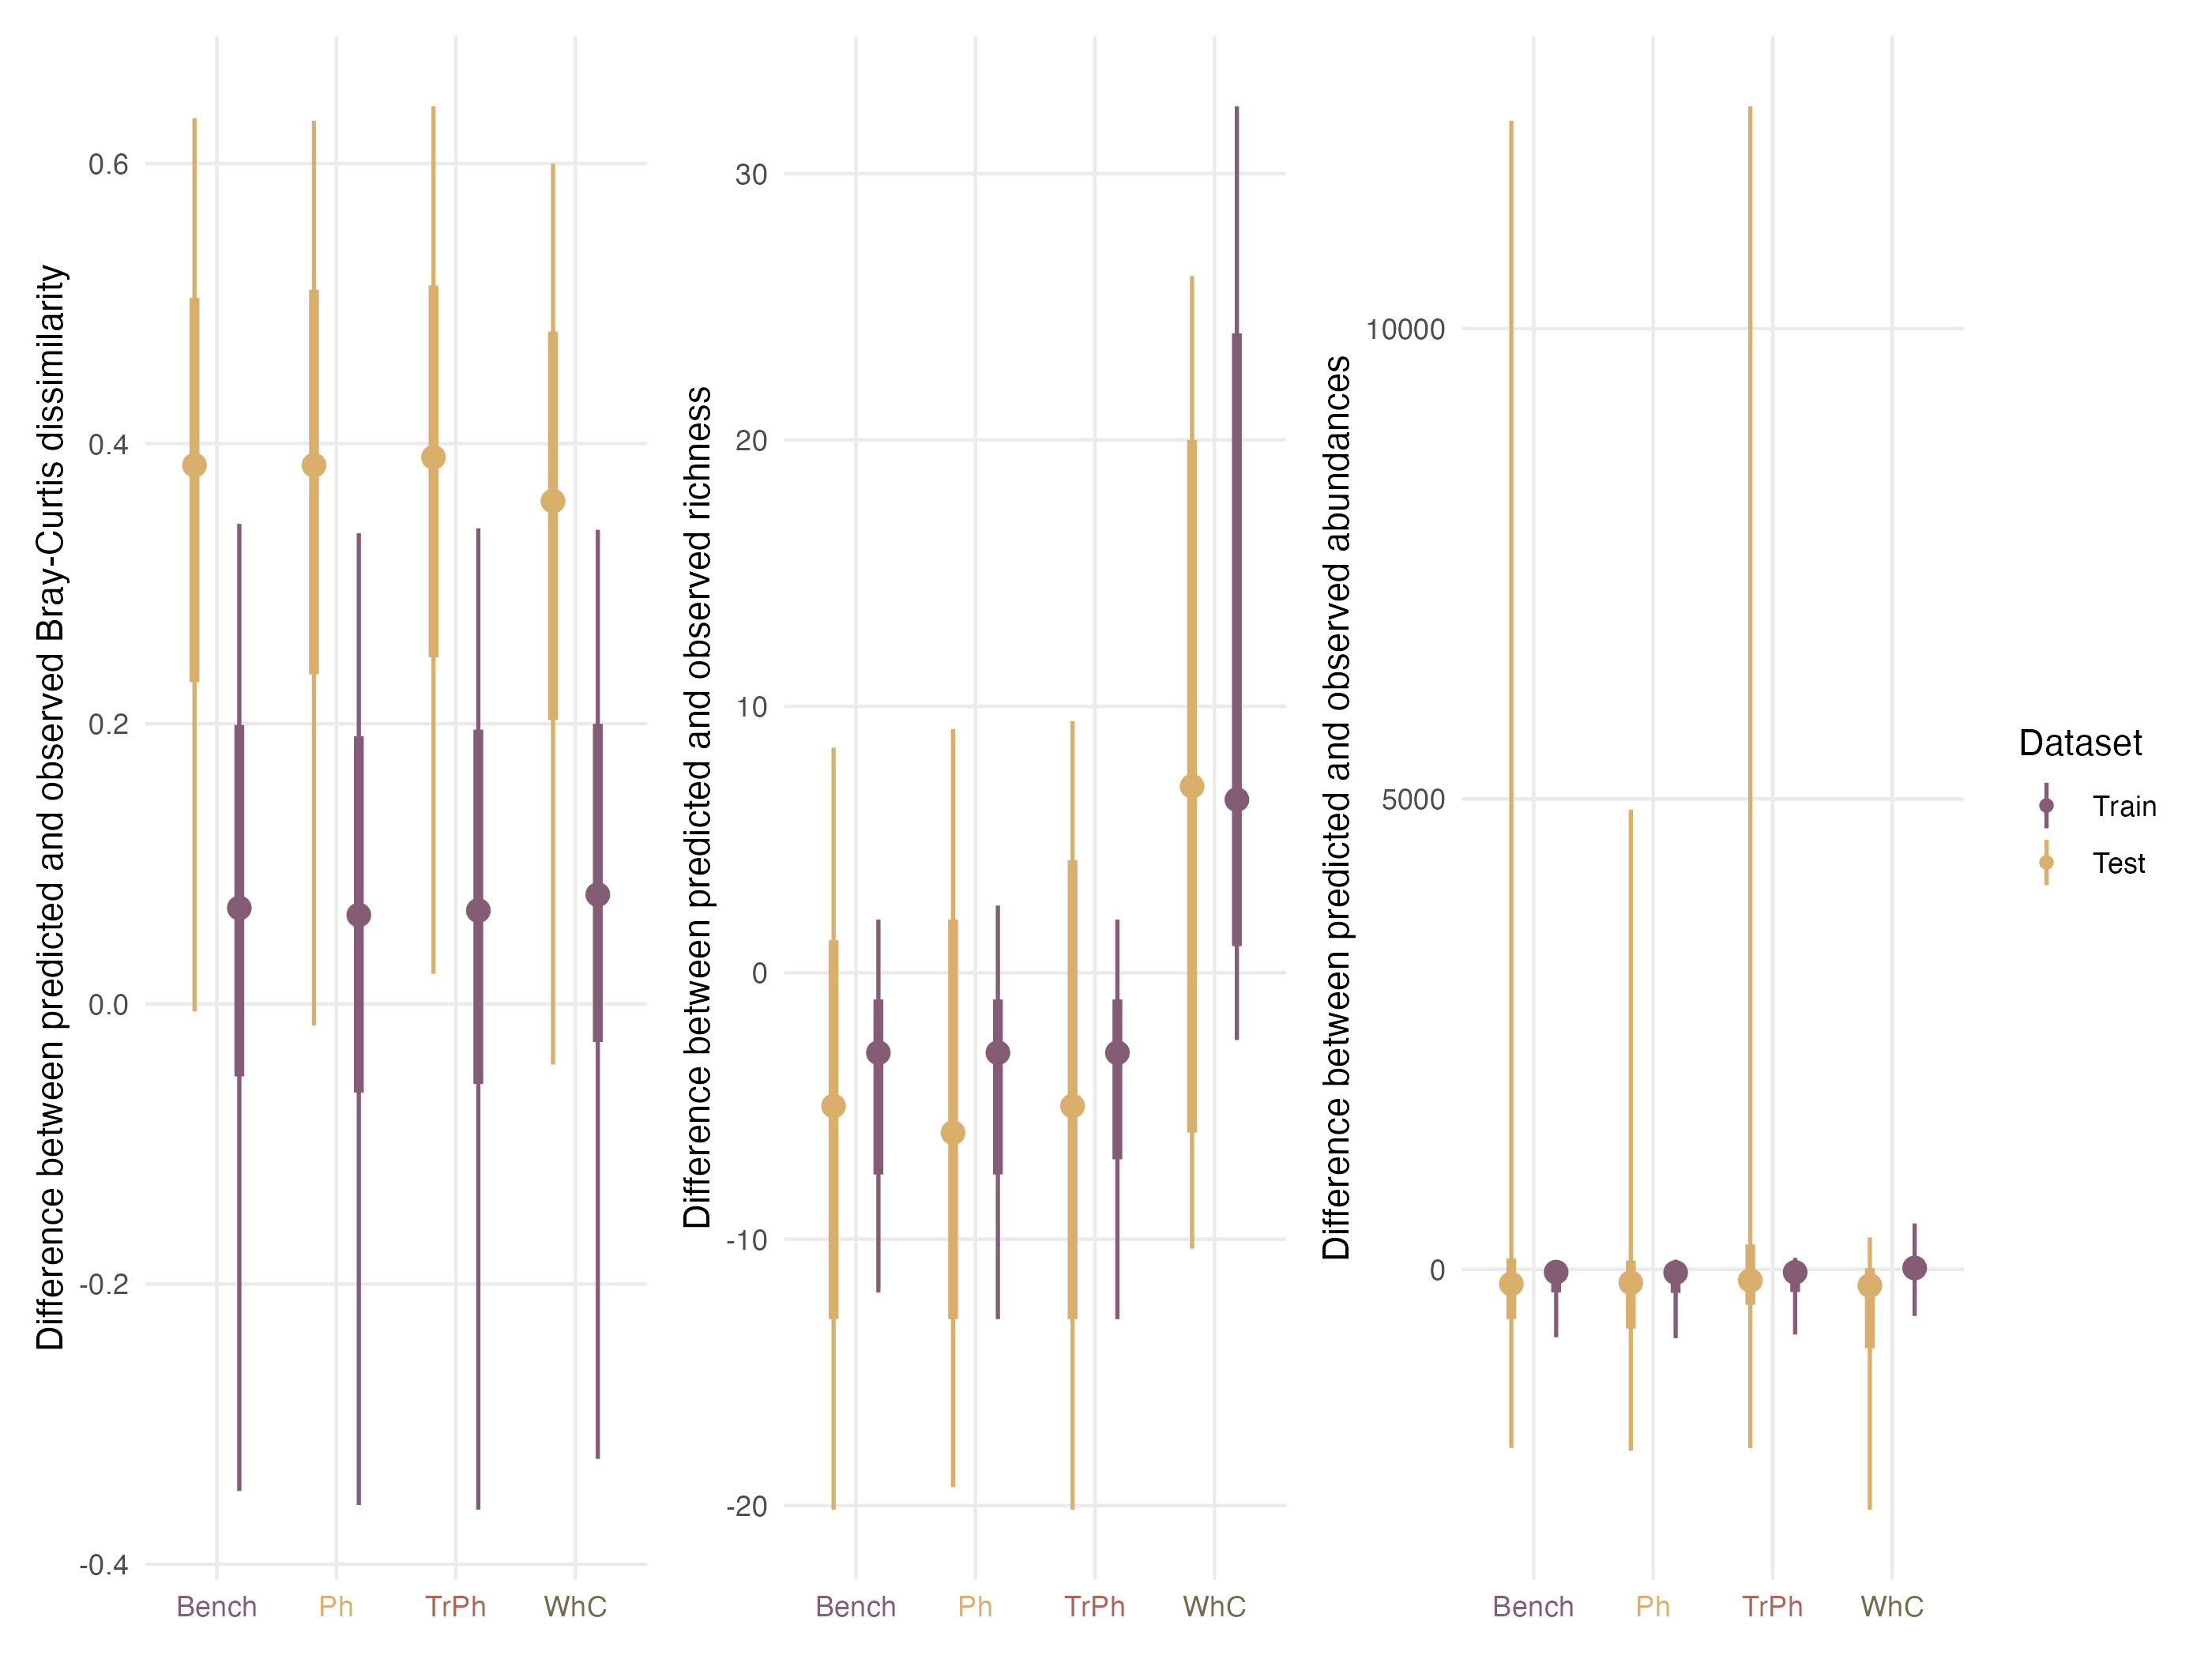
\includegraphics{figures/fig3.png}
\caption{Relative change in variance explained by environmental
predictors (left column) and by random effects (right column) power of
different model architectures with respect to the benchmark fitted with
occurrence (top line) or abundance (bottom line) data.}\label{fig:fig3}
}
\end{figure}

\hypertarget{species-niche-estimated}{%
\subsection{Species niche estimated}\label{species-niche-estimated}}

For abundance-based models, most response curves were neither convex nor
concave. For the \emph{Bench}, \emph{TrPh} and \emph{Ph} models, more
than 60\% of the estimated curves were flat, suggesting a lack of
ecologically meaningful species-environment relationships
(\cref{fig:fig4}). This rate reached more than 80\% for the \emph{WhC}
model. Other species-environment relationships included constant or
accelerated declines with \textasciitilde10\% and \textasciitilde15\% of
such shapes for the three models that do not include the whole community
(\cref{fig:fig4}). For the \emph{WhC} model, these percentages dropped
to 4.62\% and 9.24\%, respectively (\cref{fig:fig4}). Similar results
were obtained for occurence-based models (Figure S10).

\begin{figure}
\hypertarget{fig:fig4}{%
\centering
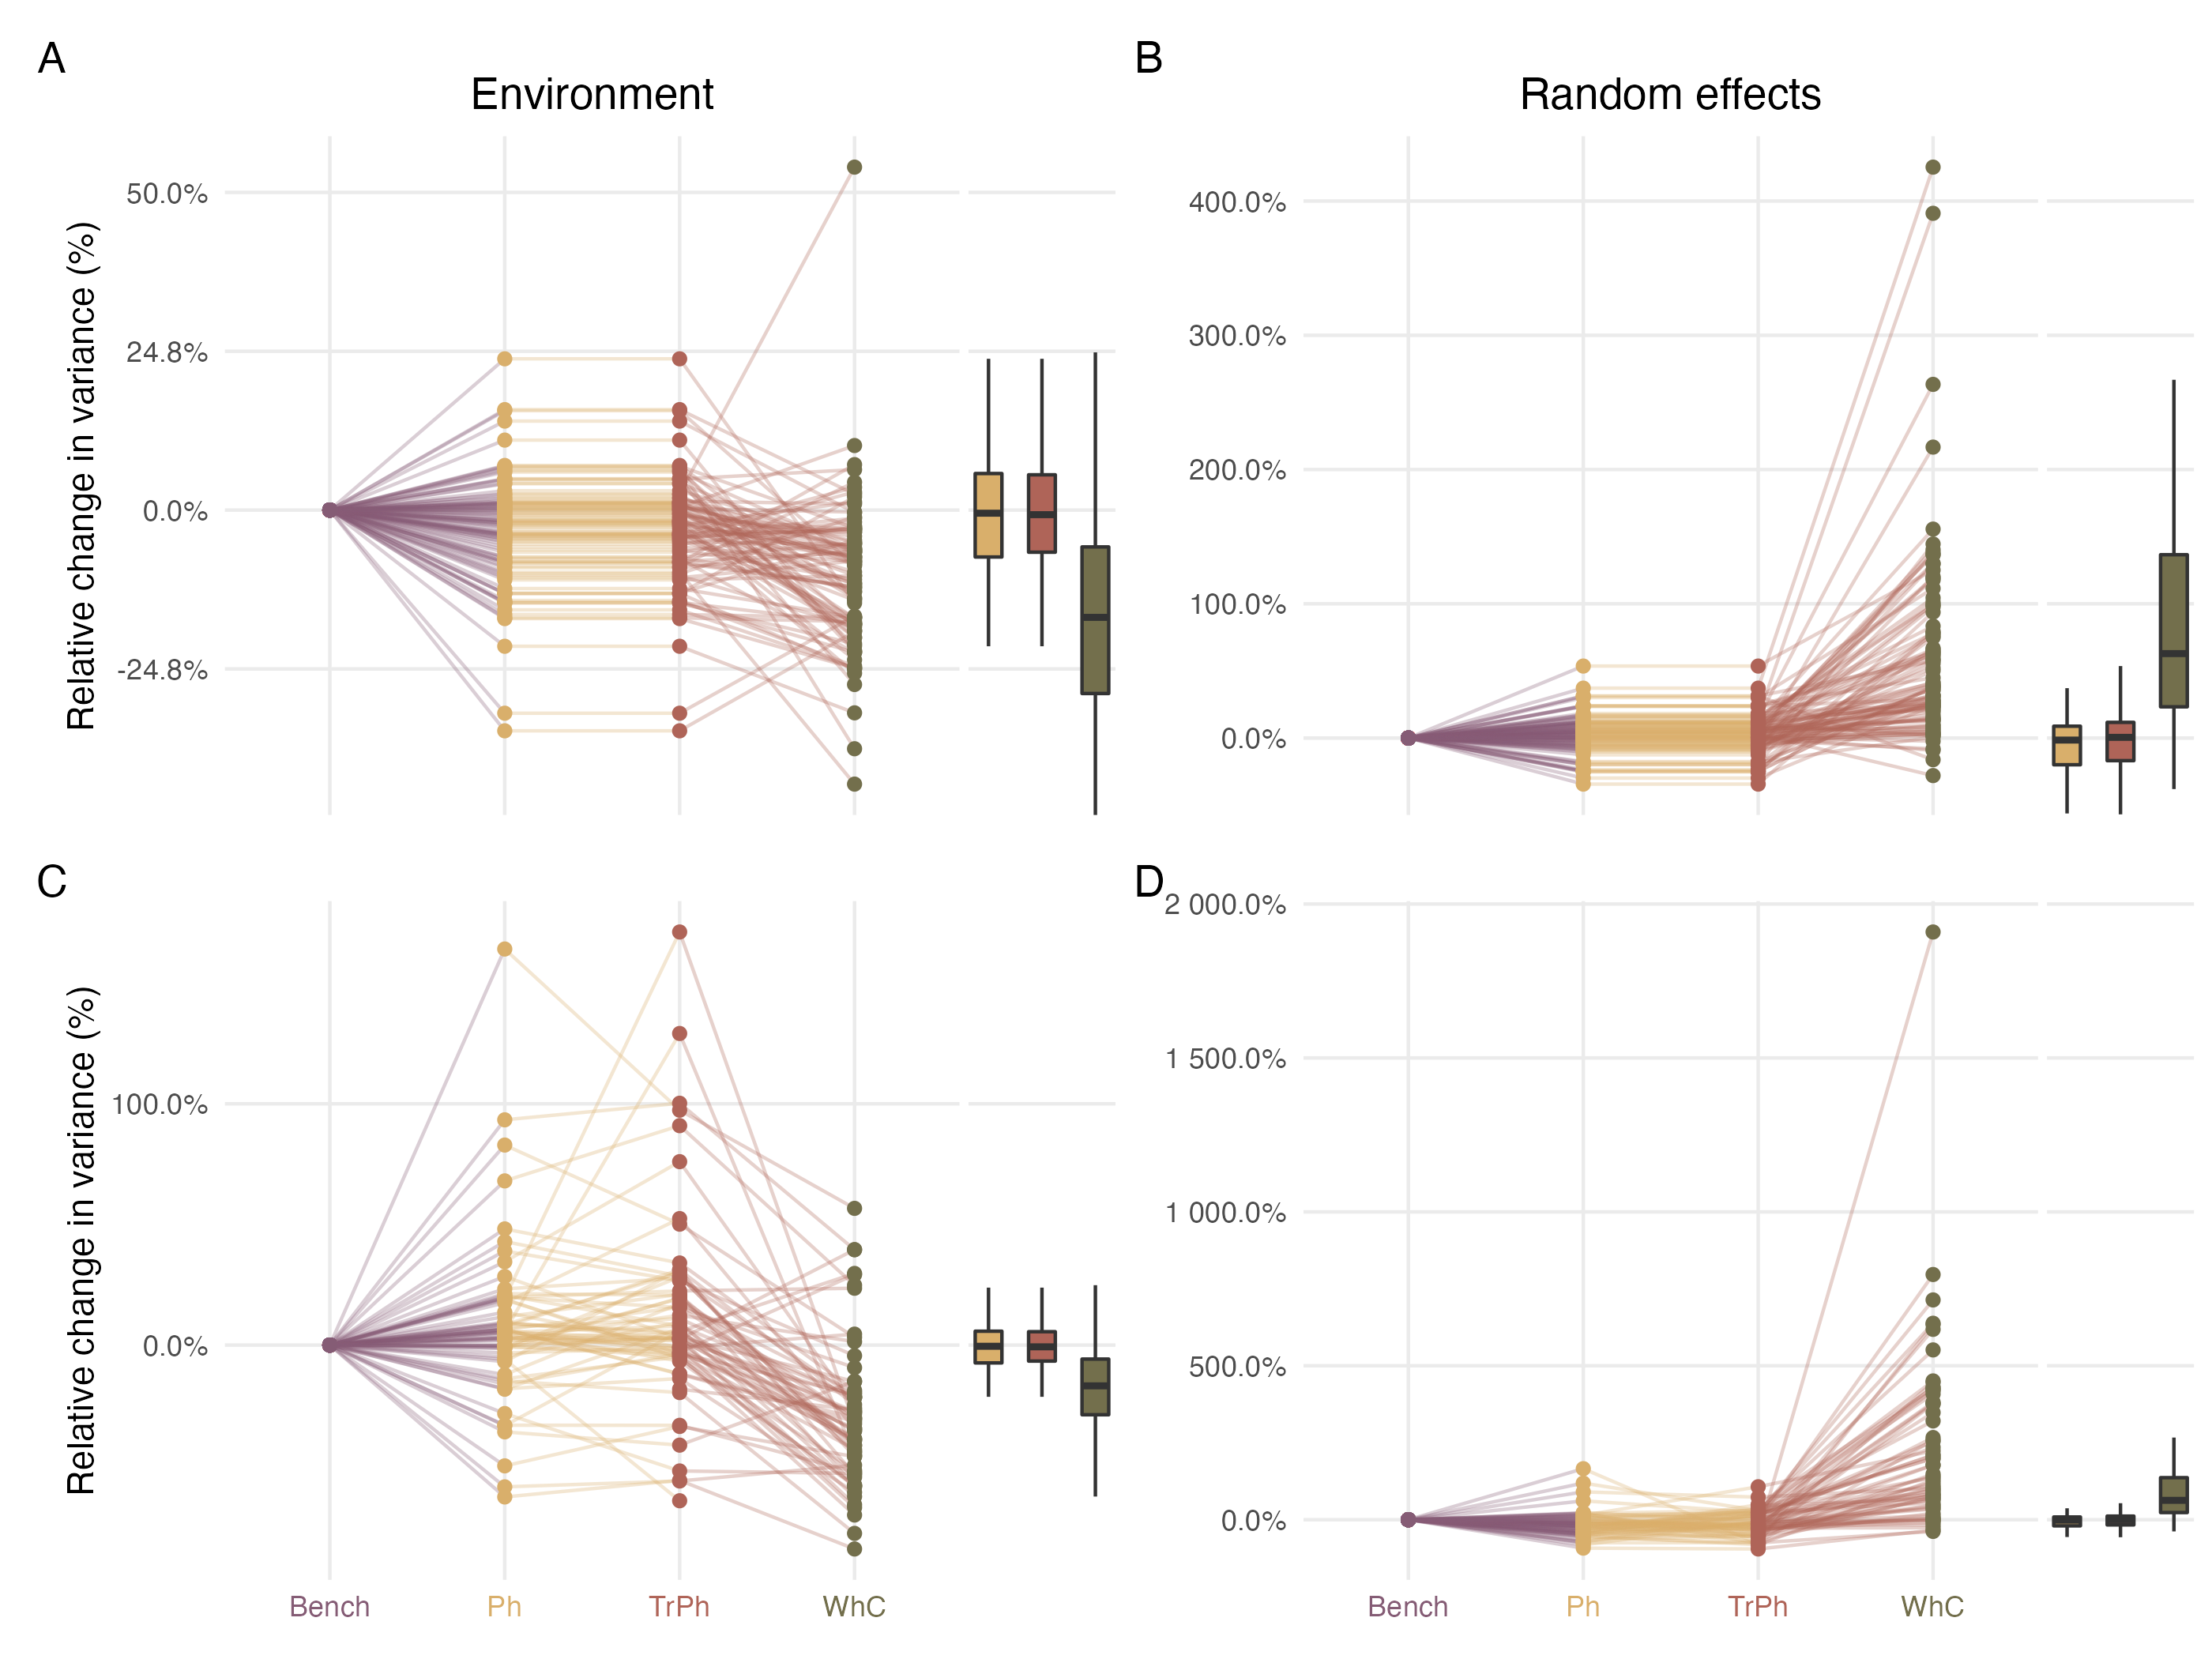
\includegraphics{figures/fig4.png}
\caption{Proportion of response curves according to the nomenclature
defined by Rigal \emph{et al.}
(\protect\hyperlink{ref-Rigal_2020}{2020}) for different model
architectures. All models have been fitted with abundance data. Each
response is characterised by a shape (column) and an intensity
(line).}\label{fig:fig4}
}
\end{figure}

Considering the \emph{TrPh} model, we further investigated the link
between the first fuzzy-PCA axis obtained from the trait matrix and the
seven environmental predictors to determine whether some traits were
favoured (or hindered) under certain environmental conditions (Figure
S6). Both abundance and occurrence-based models highlighted potentially
meaningful trait-environment relationships. For instance, mobile
predatory species were more negatively affected by fetch than sessile
suspensivore. We further found that increasing concentration in organic
matter and decreasing current velocities were associated with a higher
abundance of suspensivore populations.

\hypertarget{exploring-the-residual-correlation}{%
\subsection{Exploring the residual
correlation}\label{exploring-the-residual-correlation}}

Since all models included the same random effects, we qualitatively
compared the residual correlations estimated by the \emph{Bench} model
to the \emph{WhC} model both occurrence- and abundance-based. We
specifically considered the \emph{WhC} model for this specific
comparison, because of (1) its higher performances relative to
alternative models and (2) the larger proportion of variance explained
by the random effects in this model relative to others
(\cref{fig:fig3}).

The residual correlations estimated by the \emph{WhC} model were similar
to those estimated by the \emph{Bench} model, whether the models were
occurrence- or abundance-based (\cref{fig:fig5} and Figure S11). Yet,
the agreement between models varied depending on the random effect
considered. For instance, considering abundance-based models, the
correlation was low for random site effects (\(\text{R}^2 = 0.66\)),
moderate for random habitat effects (\(\text{R}^2 = 0.8\)) and high for
random year effects (\(\text{R}^2 = 0.91\))

\begin{figure}
\hypertarget{fig:fig5}{%
\centering
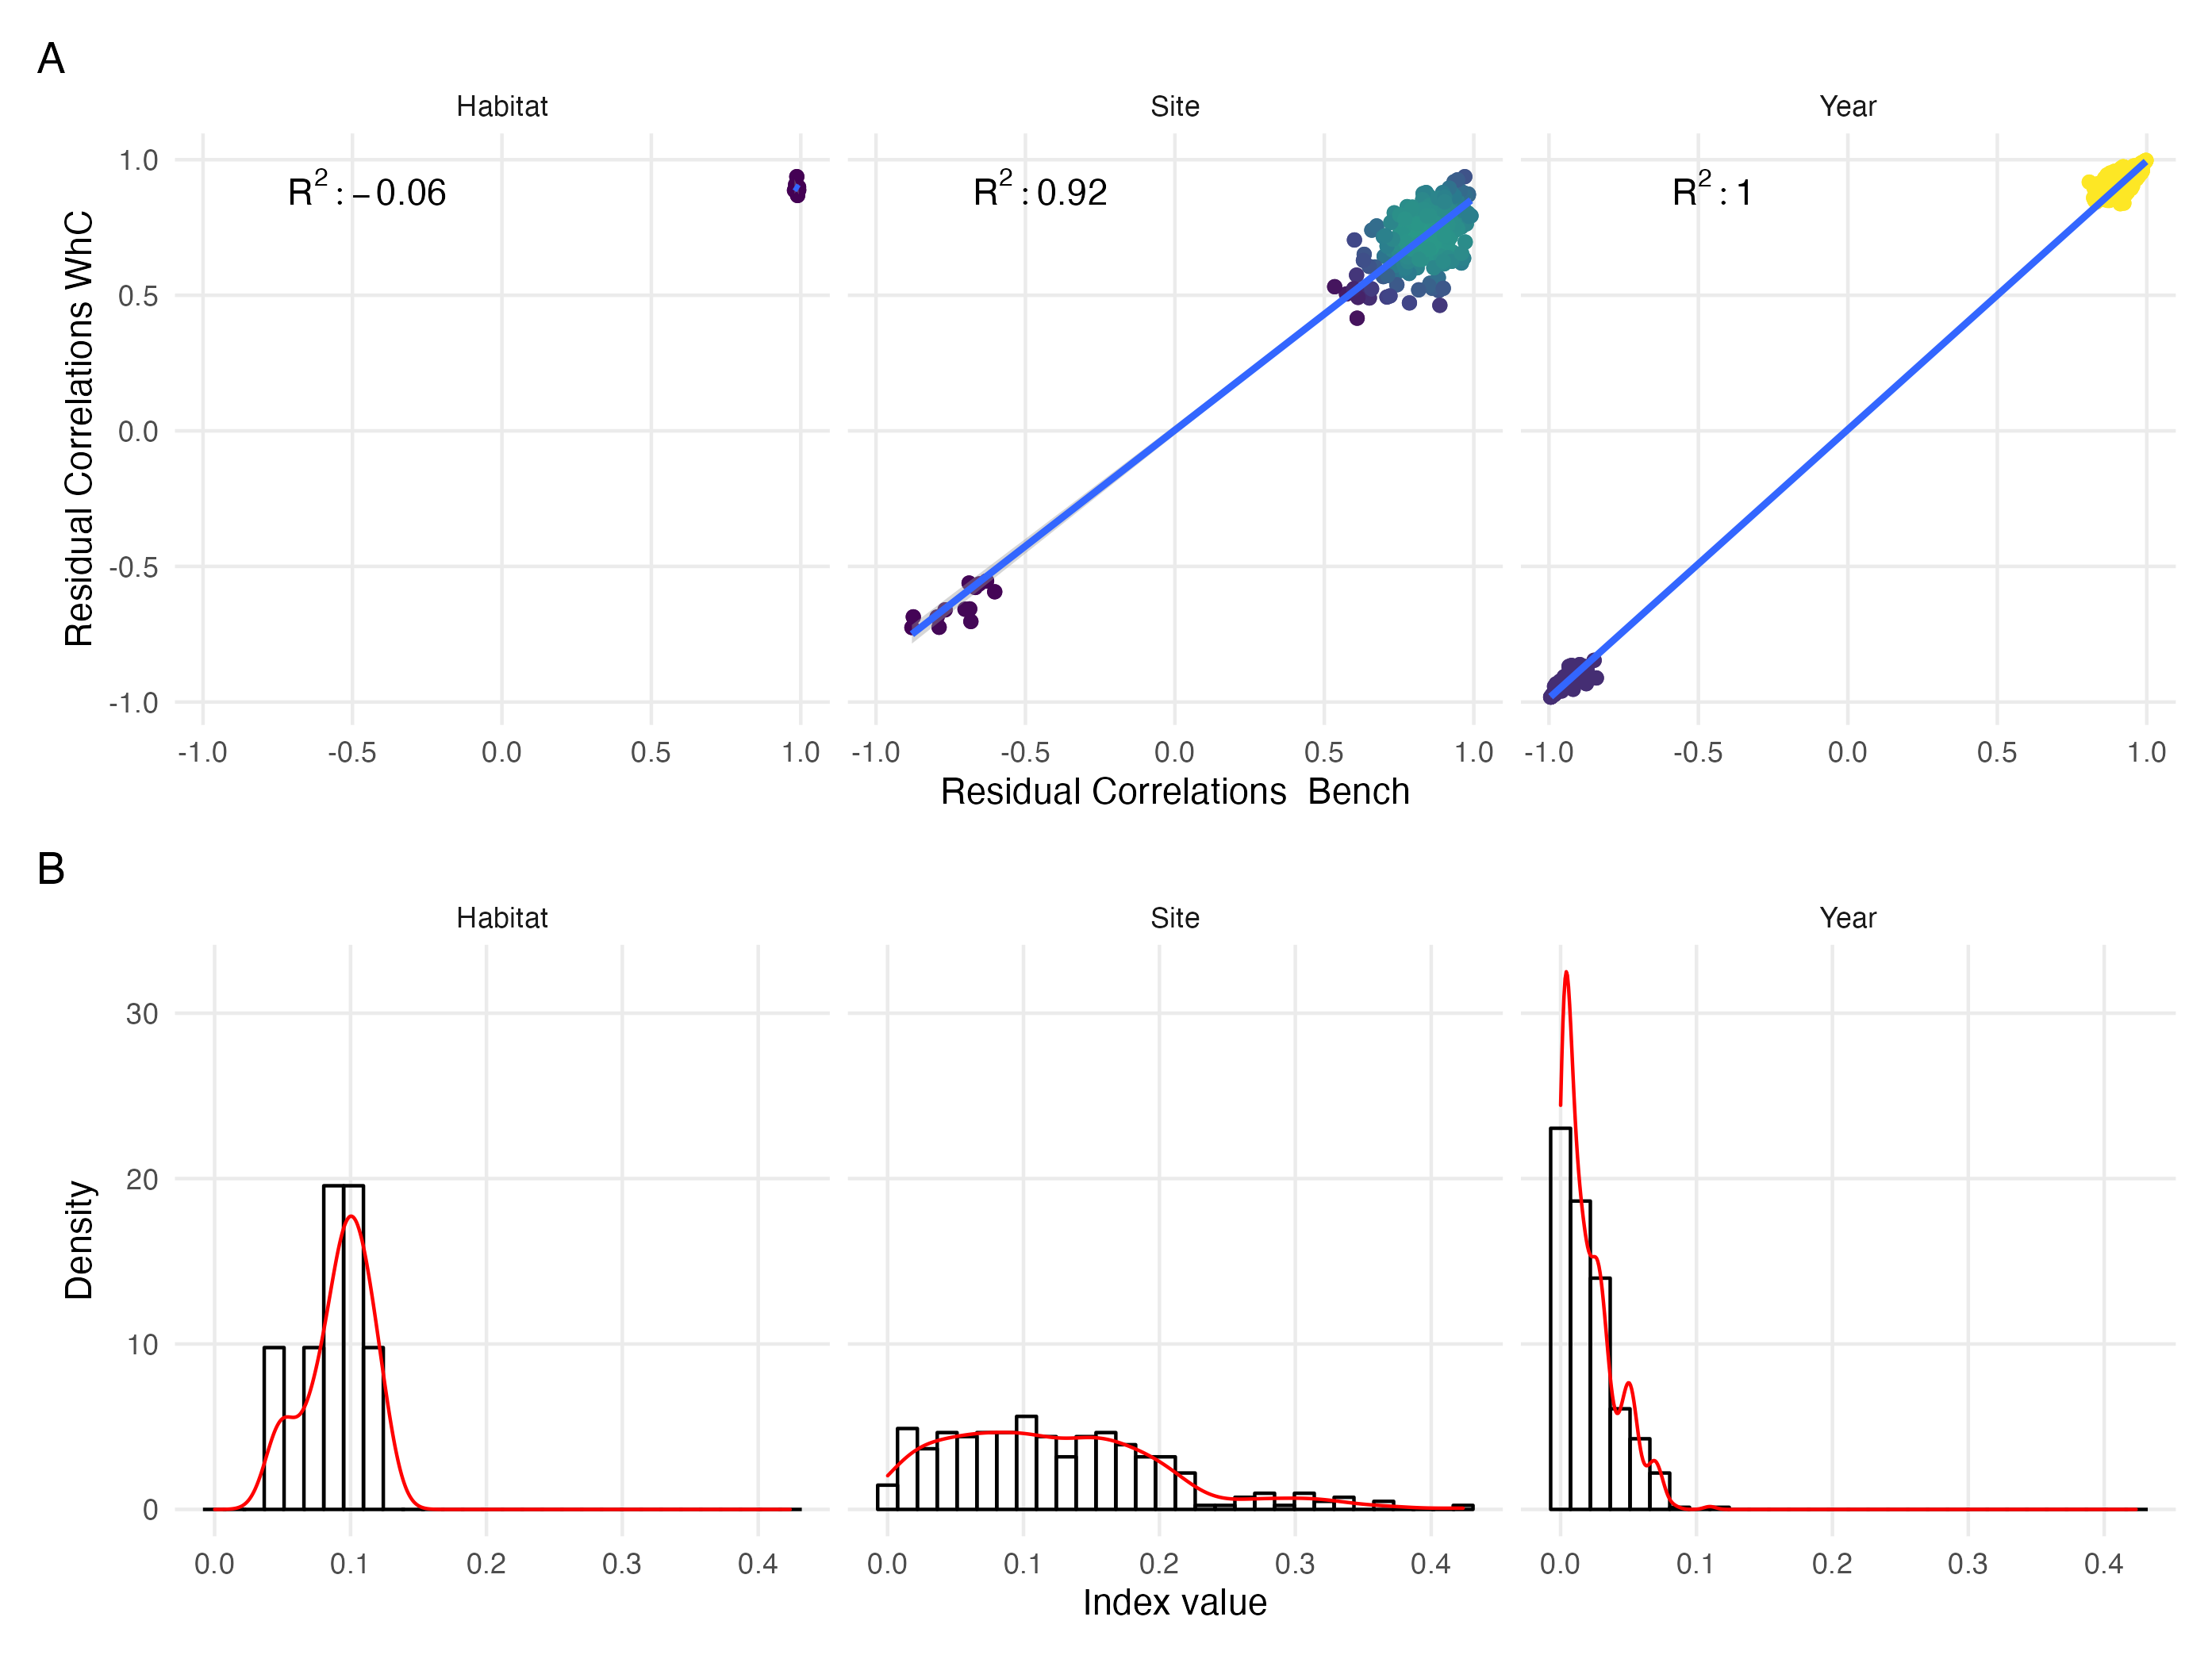
\includegraphics{figures/fig5.png}
\caption{Comparison of residual correlations estimated by Whole
Community Model and Benchmark model for the three random effect, the two
models were fitted with abundance data. A. Scatter plot of the residual
correlations estimated by the whole community model as a function of the
residual correlations estimated by the benchmark model. B. Distribution
of the index mesuring the change of sign and magnitude between residual
correlations estimated by the Whole community model and the Benchmark
model adjusted with abundance data.}\label{fig:fig5}
}
\end{figure}

Our index also qualitatively identifies the residual correlations that
have changed the most between the \emph{Bench} and \emph{WhC} models.
For abundance or occurrence-based models (\cref{fig:fig5} and Figure
S11), the mode of our index is close to zero, confirming the agreement
between the residual correlations obtained from the two models
(\cref{fig:fig5} and Figure S11). Still, our index identifies another
mode toward negative values, indicating that the sign of some
correlation coefficients have switched from positive to negative. For
abundance-based models, the random effects Habitat, Site and Year have
respectively 13.3\%, 17.7\% and 6\% of their correlation coefficients
that changed sign between the \emph{Bench} model and the \emph{WhC}
model. Similar results were obtained for occurrence-based models.

\hypertarget{discussion}{%
\section{Discussion}\label{discussion}}

It is the norm in ecological case studies to rely on partial data either
in terms of spatio-temporal resolution of monitoring data
(\protect\hyperlink{ref-Pollock_2020}{Pollock \emph{et al.} 2020}), or
in terms of available information related to target species groups
(e.g.~traits, phylogeny; Troudet \emph{et al.}
(\protect\hyperlink{ref-Troudet_2017}{2017})). In this paper we aimed to
better understand how the performance of jSDM varies depending on its
architecture, and the sources of information considered. jSDMs have two
main goals: explaining and predicting species distribution and community
composition across space and/or time
(\protect\hyperlink{ref-Tredennick_2021}{Tredennick \emph{et al.}
2021}). To date, jSDMs have mostly been tested with regards to their
predictive power (\protect\hyperlink{ref-Norberg_2019}{Norberg \emph{et
al.} 2019}), and to some extent in terms of parameter estimates
(\protect\hyperlink{ref-Wilkinson_2020}{Wilkinson \emph{et al.} 2020}),
but only when fitted on presence-absence data
(\protect\hyperlink{ref-Norberg_2019}{Norberg \emph{et al.} 2019} ;
\protect\hyperlink{ref-Wilkinson_2020}{Wilkinson \emph{et al.} 2020}).
Yet, jSDMs are increasingly fitted on abundance data (e.g. Brimacombe
\emph{et al.} (\protect\hyperlink{ref-Brimacombe_2020}{2020})) and used
for explanatory purposes (\protect\hyperlink{ref-Hakkila_2018}{Häkkilä
\emph{et al.} 2018} ; \protect\hyperlink{ref-Abrego_2016}{Abrego
\emph{et al.} 2017}). Hence, there is currently a mismatch between the
knowledge we have regarding the performance of jSDMs and their
application by ecologists. Here, we bridged both worlds using
complementary metrics and evaluation methods. Overall, we showed that
the structure of the model and the sources of information considered do
impact models' performance in many regards (e.g.~predictive power,
parameter estimates, estimated response curves, community composition).
These changes can have significant consequences on the interpretability
and the conclusions drawn from these models, especially for ecosystem
management policies.

We found that jSDM's performance increased when adding information on
the 179 accompanying species that were sampled together with the 99
polychaete species of interest. Specifically, the predictive power of
abundance-based models was considerably improved. This improvement is
likely related to the hierarchical structure of HMSC
(\protect\hyperlink{ref-Poggiato_2021}{Poggiato \emph{et al.} 2021})
where accompanying species can improve model performance by capturing a
combination of ``signals'' operating at a scale relevant for the target
community, and that can be related to the environment, to biotic
interactions, or to any other factors (e.g.~traits or and evolutionary
processes) that can help better describe the realised niche of the
species (\protect\hyperlink{ref-Ovaskainen_2017a}{Ovaskainen \emph{et
al.} 2017b}). These ``signals'' are captured by the latent residual
correlation matrix that was the feature that made jSDMs so popular at
first glance owing to its potential to be used as an indicator for
biotic interactions between species. Yet, it is now well-established
that the potential biotic signal captured by jSDMs is confounded by
other factors including a mismatch between the size of the studied
organisms and the environmental variables
(\protect\hyperlink{ref-Potter_2013}{Potter \emph{et al.} 2013}), a too
coarse spatial resolution (\protect\hyperlink{ref-Zurell_2018}{Zurell
\emph{et al.} 2018} ; \protect\hyperlink{ref-Konig_2021}{König \emph{et
al.} 2021}), or missing environmental variables
(\protect\hyperlink{ref-Dormann_2018}{Dormann \emph{et al.} 2018} ;
\protect\hyperlink{ref-Zurell_2018}{Zurell \emph{et al.} 2018} ;
\protect\hyperlink{ref-Blanchet_2020}{Blanchet \emph{et al.} 2020}).
Importantly, while including accompanying species improved predictive
performance in our case study, this does not mean that accounting for
accompanying species is always beneficial. These benefits could indeed
vary depending on the quality of the data for accompanying species
(e.g.~detection issues), their role within the ecosystem (e.g.~the case
of engineer species having a strong influence on local communities) or
the target community considered (e.g.~when the target community is
mostly under the influence of abiotic factors, then adding other species
should not have a large influence on model's performance). In practice,
most studies focus on a certain guild or taxonomic group (e.g.~fish,
birds) for data collection and/or availability reasons rather than for
ecological reasons (availability of traits or phylogeny, consistent
sampling methodology). Similarly, our choice to focus on polychaetes was
primarily guided by data availability (trait were available from Boyé
\emph{et al.} (\protect\hyperlink{ref-Boye_2019a}{2019})), although this
is a group characterised by high diversity in terms of lifestyle and
functional role (\protect\hyperlink{ref-Jumars_2015}{Jumars \emph{et
al.} 2015} ; \protect\hyperlink{ref-Giangrande_1997}{Giangrande 1997}).
Hence, most studies typically disregard the role of accompanying
species, which may bias model estimation and predictive power according
to our results. Further studies, considering a gradual increase in the
number of accompanying species, while also potentially accounting for
their trophic role or position, would help better understand the effect
of non-focal species on jSDM's performance. While communities and
assemblages remain largely defined based on arbitrary choices
(\protect\hyperlink{ref-Stroud_2015}{Stroud \emph{et al.} 2015}), such
sensitivity analysis could lead to a more objective delineation of the
appropriate ecological units to be studied (i.e.~which species are
necessary to improve model performance? Which group can be studied in
isolation?).

jSDMs have already been used to model the distribution of a wide variety
of species ranging from micro-organisms
(\protect\hyperlink{ref-Minard_2019}{Minard \emph{et al.} 2019} ;
\protect\hyperlink{ref-Pichler_2021}{Pichler \& Hartig 2021}) to
megafauna (\protect\hyperlink{ref-Rocha_2017}{Rocha \emph{et al.} 2017}
; \protect\hyperlink{ref-Brimacombe_2020}{Brimacombe \emph{et al.}
2020}) inhabiting many different ecosystems. Here, while we studied
communities associated with two typical coastal habitats, i.e.~seagrass
and sand, that have original characteristics as they are located at the
land-sea interface (\protect\hyperlink{ref-Boye_2019a}{Boyé \emph{et
al.} 2019}), our case study reflects typical aspects of data in
ecological research such as data limitation and data availability but
also typical aspects of the functioning and structure of communities
(e.g.~prevalence of rare and transient species; Magurran \& Henderson
(\protect\hyperlink{ref-Magurran_2003}{n.d.}) ; Snell Taylor \emph{et
al.} (\protect\hyperlink{ref-SnellTaylor_2018}{2018})). Our results
provide a few insights on trait-environment relationships but we suspect
that trait data quality and availability remains limiting to fully
exploit what functional ecology can bring to jSDMs
(\protect\hyperlink{ref-Tyler_2012}{Tyler \emph{et al.} 2012} ;
\protect\hyperlink{ref-deJuan_2022}{Juan \emph{et al.} 2022}). For
instance, we found an interaction between trophic modalities
(i.e.~microphagous versus macrophagous diet) and fetch (Fig. S15), which
indicates that organisms that filter on small particles are less likely
to occur in wave-exposed sites where high levels of sediment
resuspension can block their filtering systems
(\protect\hyperlink{ref-Manning_2014}{LM \emph{et al.} 2014});
conversely macrophagous organisms are less impacted by fetch. Yet, most
trait-environment relationships, and most species-environment
relationships were flat; a result that could reflect a symptom of the
functioning of the system, where neutral processes are expected to
dominate (e.g.~in seagrass bed communities, Boyé \emph{et al.}
(\protect\hyperlink{ref-Boye_2019a}{2019})). However, the lack of
contribution of other trait-environment relationships in our model could
also be related to a mismatch between trait data, environmental data,
and the ecological processes at play. For instance, the physical coastal
environment is highly dynamic; a feature that is only partially
characterised by our environmental variables that summarise average
climatological conditions (but not extreme events or annual/seasonal
variability). Likewise, the list of available fuzzy-coded traits only
partially captures species capacity to adapt to frequent disturbances or
environmental variability (\protect\hyperlink{ref-Violle_2012}{Violle
\emph{et al.} 2012} ; \protect\hyperlink{ref-deJuan_2022}{Juan \emph{et
al.} 2022}). Most studies will face the same trade-off between the
potential benefit of including traits within jSDMs and the effort needed
to collect relevant information. In our case, while including traits did
not improve the model's predictive power, it provides knowledge that is
useful to understand the response of species along environmental
gradients, and set-up management strategies. Hence, if the goal is not
prediction but inference
(\protect\hyperlink{ref-Tredennick_2021}{Tredennick \emph{et al.}
2021}), including traits and proxies of phylogeny might still be useful
to interpret the models, provided that explanatory power is not affected
(as in our case), and that computation time is not too cumbersome given
the added parameters.

Understanding the behaviour of increasingly complex models from a
mathematical and ecological point of view is one of the major challenges
currently facing numerical ecology and one active research area
(\protect\hyperlink{ref-Lucas_2020}{Lucas 2020} ;
\protect\hyperlink{ref-Ryo_2021}{Ryo \emph{et al.} 2021}). jSDMs can be
particularly difficult to interpret because the number of parameters
drastically increases with the size of the community (the curse of
dimensionality; Tikhonov \emph{et al.}
(\protect\hyperlink{ref-Tikhonov_2017}{2017})). Combined with the use of
latent variables, auditing this type of model is very complex, and
requires a diverse set of metrics
(\protect\hyperlink{ref-Wilkinson_2020}{Wilkinson \emph{et al.} 2020}),
notably to understand what is hidden in the signal captured by the
residual correlations between species. While guidelines have been
developed to characterise the performance of jSDM fitted on occurrence
data (\protect\hyperlink{ref-Wilkinson_2020}{Wilkinson \emph{et al.}
2020}), it is only recently that the predictive power of abundance-based
models has been explored Waldock \emph{et al.}
(\protect\hyperlink{ref-Waldock_2022}{2022}). Here, we used a set of
complementary metrics to assess the performance of both occurrence- and
abundance-based models at the species and community levels, the latter
considering both alpha and beta diversity. We also transposed a method
initially developed for time series
(\protect\hyperlink{ref-Rigal_2020}{Rigal \emph{et al.} 2020}) to
provide an innovative way of characterising the response curves of each
species. Further, we bring together a set of approaches and propose a
new index to characterise and compare residual correlations networks.
Overall, we provide a comprehensive framework ultimately allowing for an
integrative assessment and comparison of jSDM performance.

As our models performed equally well in terms of explanatory power, it
is important to ask whether and to which extent adding extra information
is beneficial to jSDM models. Adding accompanying species has two main
benefits : increasing predictive power and clarifying
species-environment relationships. For the former, while the predictive
power was improved by taking the whole community into account, the gain
remained small. Hence, if the objective is prediction, machine learning
or neural networks applied to community data may provide an interesting
alternative to jSDM (\protect\hyperlink{ref-Zhang_2020}{Zhang \emph{et
al.} 2020} ; \protect\hyperlink{ref-Deneu_2021}{Deneu \emph{et al.}
2021}). Still, jSDMs provide an interesting compromise between
predictive power and interpretability
(\protect\hyperlink{ref-Norberg_2019}{Norberg \emph{et al.} 2019} ;
\protect\hyperlink{ref-Ovaskainen_2017a}{Ovaskainen \emph{et al.}
2017b}) and adding accompanying species could prove a useful strategy
for informing conservation through community models
(\protect\hyperlink{ref-Pollock_2020}{Pollock \emph{et al.} 2020}). For
the latter, adding accompanying species helped clarify and remove
spurious species-environment relationships (many switching from
non-linear responses to flat ones). Nonetheless, it is important to keep
in mind that the more species you add, the more weight they have in the
likelihood and therefore on the estimated species-environment
relationships. Thus if the purpose is inference, adding more species may
not be the best strategy. Adding trait information or phylogeny seems
more appropriate as it leads to more interpretable models. Overall, our
results provide new insights into the most appropriate strategies for
jSDM fitting, according to the objective of the modelling exercise
(\protect\hyperlink{ref-Troudet_2017}{Troudet \emph{et al.} 2017}) and
the data at hand. Future work could expand on other ecosystems
presenting different characteristics (e.g., with stronger environmental
filters or competitive processes) or use simulations
(\protect\hyperlink{ref-Zurell_2010}{Zurell \emph{et al.} 2010}) to
confirm the generality of our findings.

\hypertarget{author-contributions}{%
\subsection{Author Contributions}\label{author-contributions}}

All authors conceived thes ideas and Violet, Boyé, Chevalier and
Marzloff designed the methodology; Boyé, Grall and Gauthier provided the
data; Violet analysed the data; Violet, Boyé, Chevalier and Marzloff led
the writing of the manuscript. All authors contributed critically to the
drafts and gave final approval for publication.

\hypertarget{acknowledgment}{%
\subsection{Acknowledgment}\label{acknowledgment}}

The authors acknowledge the Pôle de Calcul et de Données Marines (PCDM)
for providing DATARMOR storage and computational resources.
\url{https://pcdm.ifremer.fr}

\hypertarget{conflict-of-interest}{%
\subsection{Conflict of interest}\label{conflict-of-interest}}

The authors declare no conflict of interest.

\hypertarget{references}{%
\section*{References}\label{references}}
\addcontentsline{toc}{section}{References}

\hypertarget{refs}{}
\begin{CSLReferences}{1}{0}
\leavevmode\vadjust pre{\hypertarget{ref-Abrego_2016}{}}%
Abrego, N., Dunson, D., Halme, P., Salcedo, I. \& Ovaskainen, O. (2017).
\href{https://doi.org/10.1111/oik.03674}{Wood-inhabiting fungi with
tight associations with other species have declined as a response to
forest management}. \emph{Oikos}, 126.

\leavevmode\vadjust pre{\hypertarget{ref-Baselga_2010}{}}%
Baselga, A. (2010).
\href{https://doi.org/10.1111/j.1466-8238.2009.00490.x}{Partitioning the
turnover and nestedness components of beta diversity}. \emph{Global
Ecology and Biogeography}, 19, 134--143.

\leavevmode\vadjust pre{\hypertarget{ref-Baselga_2022}{}}%
Baselga, A., Orme, D., Villeger, S., De Bortoli, J., Leprieur, F. \&
Logez, M. (2022).
\emph{\href{https://CRAN.R-project.org/package=betapart}{betapart:
Partitioning Beta Diversity into Turnover and Nestedness Components}}.

\leavevmode\vadjust pre{\hypertarget{ref-Blanchet_2020}{}}%
Blanchet, F.G., Cazelles, K. \& Gravel, D. (2020).
\href{https://doi.org/10.1111/ele.13525}{Co-occurrence is not evidence
of ecological interactions}. \emph{Ecology Letters}.

\leavevmode\vadjust pre{\hypertarget{ref-Boye_2019b}{}}%
Boyé, A. (2019). Diversité taxinomique et fonctionnelle des habitats
benthiques dans l'espace et dans le temps: une perspective régionale et
décennale. thèse de doctorat. Université de Bretagne Occidentale,
Université de Montréal.

\leavevmode\vadjust pre{\hypertarget{ref-Boye_2017}{}}%
Boyé, A., Legendre, P., Grall, J. \& Gauthier, O. (2017).
\href{https://doi.org/10.1016/j.seares.2017.06.004}{Constancy despite
variability: Local and regional macrofaunal diversity in intertidal
seagrass beds}. \emph{Journal of Sea Research}, 130, 107--122.

\leavevmode\vadjust pre{\hypertarget{ref-Boye_2019a}{}}%
Boyé, A., Thiébaut, Éric, Grall, J., Legendre, P., Broudin, C., Houbin,
C., \emph{et al.} (2019).
\href{https://doi.org/10.1111/ddi.12987}{Trait-based approach to
monitoring marine benthic data along 500 km of coastline}.
\emph{Diversity and Distributions}, 25, 1879--1896.

\leavevmode\vadjust pre{\hypertarget{ref-Brimacombe_2020}{}}%
Brimacombe, C., Bodner, K. \& Fortin, M.-J. (2020).
\href{https://doi.org/10.1111/ecog.05452}{Inferred seasonal interaction
rewiring of a freshwater stream fish network}. \emph{Ecography}, n/a.

\leavevmode\vadjust pre{\hypertarget{ref-Brudvig_2022}{}}%
Brudvig, L.A. \& Catano, C.P. (2022).
\href{https://doi.org/10.1111/rec.13380}{Prediction and uncertainty in
restoration science}. \emph{Restoration Ecology}, n/a, e13380.

\leavevmode\vadjust pre{\hypertarget{ref-Chesson_2000}{}}%
Chesson, P. (2000).
\href{https://doi.org/10.1146/annurev.ecolsys.31.1.343}{Mechanisms of
Maintenance of Species Diversity}. \emph{Annual Review of Ecology and
Systematics}, 31, 343--366.

\leavevmode\vadjust pre{\hypertarget{ref-Chiquet_2021}{}}%
Chiquet, J., Mariadassou, M. \& Robin, S. (2021).
\href{https://doi.org/10.3389/fevo.2021.588292}{The Poisson-Lognormal
Model as a Versatile Framework for the Joint Analysis of Species
Abundances}. \emph{Frontiers in Ecology and Evolution}, 9.

\leavevmode\vadjust pre{\hypertarget{ref-Deneu_2021}{}}%
Deneu, B., Servajean, M., Bonnet, P., Botella, C., Munoz, F. \& Joly, A.
(2021). Convolutional neural networks improve species distribution
modelling by capturing the spatial structure of the environment.
\emph{PLoS Computational Biology}.

\leavevmode\vadjust pre{\hypertarget{ref-Dietze_2018}{}}%
Dietze, M.C., Fox, A., Beck-Johnson, L.M., Betancourt, J.L., Hooten,
M.B., Jarnevich, C.S., \emph{et al.} (2018).
\href{https://doi.org/10.1073/pnas.1710231115}{Iterative near-term
ecological forecasting: Needs, opportunities, and challenges}.
\emph{Proceedings of the National Academy of Sciences}, 115, 1424--1432.

\leavevmode\vadjust pre{\hypertarget{ref-Dormann_2018}{}}%
Dormann, C.F., Bobrowski, M., Dehling, D.M., Harris, D.J., Hartig, F.,
Lischke, H., \emph{et al.} (2018).
\href{https://doi.org/10.1111/geb.12759}{Biotic interactions in species
distribution modelling: 10 questions to guide interpretation and avoid
false conclusions}. \emph{Global Ecology and Biogeography}, 27,
1004--1016.

\leavevmode\vadjust pre{\hypertarget{ref-Dunn_1964}{}}%
Dunn, O.J. (1964).
\href{https://doi.org/10.1080/00401706.1964.10490181}{Multiple
Comparisons Using Rank Sums}. \emph{Technometrics}, 6, 241--252.

\leavevmode\vadjust pre{\hypertarget{ref-Elith_2006}{}}%
Elith, J., H. Graham, C., P. Anderson, R., Dudı́k, M., Ferrier, S.,
Guisan, A., \emph{et al.} (2006).
\href{https://doi.org/10.1111/j.2006.0906-7590.04596.x}{Novel methods
improve prediction of species' distributions from occurrence data}.
\emph{Ecography}, 29, 129--151.

\leavevmode\vadjust pre{\hypertarget{ref-Gelman_2020}{}}%
Gelman, A., Hill, J. \& Vehtari, A. (2020).
\emph{\href{https://doi.org/10.1017/9781139161879}{Regression and Other
Stories}}. Analytical Methods for Social Research. Cambridge University
Press.

\leavevmode\vadjust pre{\hypertarget{ref-Gelman_1992}{}}%
Gelman, A. \& Rubin, D.B. (1992).
\href{https://doi.org/10.1214/ss/1177011136}{Inference from Iterative
Simulation Using Multiple Sequences}. \emph{Statistical Science}, 7,
457--472.

\leavevmode\vadjust pre{\hypertarget{ref-Giangrande_1997}{}}%
Giangrande, A. (1997).
\href{https://doi.org/10.1201/b12590-8}{Polychaete reproductive
patterns, life cycles and life histories: an overview}. In:
\emph{Oceanography And Marine Biology} (ed. A. D.Ansell, M.B., R.
N.Gibson). CRC Press, pp. 310--411.

\leavevmode\vadjust pre{\hypertarget{ref-Giangrande_2005}{}}%
Giangrande, A., Licciano, M. \& Musco, L. (2005).
\href{https://doi.org/10.1016/j.marpolbul.2005.08.003}{Polychaetes as
environmental indicators revisited}. \emph{Marine Pollution Bulletin},
50, 1153--1162.

\leavevmode\vadjust pre{\hypertarget{ref-Giannini_2013}{}}%
Giannini, T.C., Chapman, D.S., Saraiva, A.M., Alves-dos-Santos, I. \&
Biesmeijer, J.C. (2013).
\href{https://doi.org/10.1111/j.1600-0587.2012.07191.x}{Improving
species distribution models using biotic interactions: a case study of
parasites, pollinators and plants}. \emph{Ecography}, 36, 649--656.

\leavevmode\vadjust pre{\hypertarget{ref-Godsoe_2017}{}}%
Godsoe, W., Franklin, J. \& Blanchet, F.G. (2017).
\href{https://doi.org/10.1002/ece3.2657}{Effects of biotic interactions
on modeled species' distribution can be masked by environmental
gradients}. \emph{Ecology and Evolution}, 7, 654--664.

\leavevmode\vadjust pre{\hypertarget{ref-Hakkila_2018}{}}%
Häkkilä, M., Abrego, N., Ovaskainen, O. \& Mönkkönen, M. (2018).
\href{https://doi.org/10.1002/ece3.3923}{Habitat quality is more
important than matrix quality for bird communities in protected areas}.
\emph{Ecology and Evolution}, 8, 4019--4030.

\leavevmode\vadjust pre{\hypertarget{ref-Holt_2020}{}}%
Holt, R.D. (2020). \href{https://doi.org/10.17161/bi.v15i1.13302}{Some
thoughts about the challenge of inferring ecological interactions from
spatial data.} \emph{Biodiversity Informatics}, 15, 61--66.

\leavevmode\vadjust pre{\hypertarget{ref-Houlahan_2017}{}}%
Houlahan, J.E., McKinney, S.T., Anderson, T.M. \& McGill, B.J. (2017).
\href{https://doi.org/10.1111/oik.03726}{The priority of prediction in
ecological understanding}. \emph{Oikos}, 126, 1--7.

\leavevmode\vadjust pre{\hypertarget{ref-Howard_2014}{}}%
Howard, C., Stephens, P.A., Pearce-Higgins, J.W., Gregory, R.D. \&
Willis, S.G. (2014).
\href{https://doi.org/10.1111/2041-210X.12184}{Improving species
distribution models: the value of data on abundance}. \emph{Methods in
Ecology and Evolution}, 5, 506--513.

\leavevmode\vadjust pre{\hypertarget{ref-Hui_2016}{}}%
Hui, F.K.C. (2016). \href{https://doi.org/10.1111/2041-210X.12514}{boral
-- Bayesian Ordination and Regression Analysis of Multivariate Abundance
Data in r}. \emph{Methods in Ecology and Evolution}, 7, 744--750.

\leavevmode\vadjust pre{\hypertarget{ref-ipbes_2019}{}}%
IPBES. (2019). \href{https://doi.org/10.5281/zenodo.6417333}{Global
assessment report on biodiversity and ecosystem services of the
Intergovernmental Science-Policy Platform on Biodiversity and Ecosystem
Services}.

\leavevmode\vadjust pre{\hypertarget{ref-Ives_2011}{}}%
Ives, A.R. \& Helmus, M.R. (2011).
\href{https://doi.org/10.1890/10-1264.1}{Generalized linear mixed models
for phylogenetic analyses of community structure}. \emph{Ecological
Monographs}, 81, 511--525.

\leavevmode\vadjust pre{\hypertarget{ref-deJuan_2022}{}}%
Juan, S. de, Bremner, J., Hewitt, J., Törnroos, A., Mangano, M.C.,
Thrush, S., \emph{et al.} (2022).
\href{https://doi.org/10.1002/ece3.9001}{Biological traits approaches in
benthic marine ecology: Dead ends and new paths}. \emph{Ecology and
Evolution}, 12, e9001.

\leavevmode\vadjust pre{\hypertarget{ref-Jumars_2015}{}}%
Jumars, P.A., Dorgan, K.M. \& Lindsay, S.M. (2015).
\href{https://doi.org/10.1146/annurev-marine-010814-020007}{Diet of
Worms Emended: An Update of Polychaete Feeding Guilds}. \emph{Annual
Review of Marine Science}, 7, 497--520.

\leavevmode\vadjust pre{\hypertarget{ref-Keil_2021}{}}%
Keil, P., Wiegand, T., Tóth, A.B., McGlinn, D.J. \& Chase, J.M. (2021).
\href{https://doi.org/10.1002/ecm.1452}{Measurement and analysis of
interspecific spatial associations as a facet of biodiversity}.
\emph{Ecological Monographs}, n/a.

\leavevmode\vadjust pre{\hypertarget{ref-Konig_2021}{}}%
König, C., Wüest, R.O., Graham, C.H., Karger, D.N., Sattler, T.,
Zimmermann, N.E., \emph{et al.} (2021).
\href{https://doi.org/10.1111/jbi.14106}{Scale dependency of joint
species distribution models challenges interpretation of biotic
interactions}. \emph{Journal of Biogeography}, 48, 1541--1551.

\leavevmode\vadjust pre{\hypertarget{ref-Levine_2017}{}}%
Levine, J.M., Bascompte, J., Adler, P.B. \& Allesina, S. (2017).
\href{https://doi.org/10.1038/nature22898}{Beyond pairwise mechanisms of
species coexistence in complex communities}. \emph{Nature}, 546, 56--64.

\leavevmode\vadjust pre{\hypertarget{ref-Manning_2014}{}}%
LM, M., CH, P. \& MJ, B. (2014).
\href{https://www.int-res.com/abstracts/meps/v508/p1-15/}{Dominant
macrobenthic populations experience sustained impacts from annual
disposal of fine sediments on sandy beaches}. \emph{Marine Ecology
Progress Series}, 508, 1--15.

\leavevmode\vadjust pre{\hypertarget{ref-Lucas_2020}{}}%
Lucas, T.C.D. (2020). \href{https://doi.org/10.1002/ecm.1422}{A
translucent box: interpretable machine learning in ecology}.
\emph{Ecological Monographs}, 90, e01422.

\leavevmode\vadjust pre{\hypertarget{ref-Magurran_2003}{}}%
Magurran, A.E. \& Henderson, P.A. (n.d.).
\href{https://doi.org/10.1038/nature01547}{Explaining the excess of rare
species in natural species abundance distributions}. \emph{Nature}, 422,
714--716.

\leavevmode\vadjust pre{\hypertarget{ref-Minard_2019}{}}%
Minard, G., Tikhonov, G., Ovaskainen, O. \& Saastamoinen, M. (2019).
\href{https://doi.org/10.1111/1462-2920.14786}{The microbiome of the
Melitaea cinxia butterfly shows marked variation but is only little
explained by the traits of the butterfly or its host plant}.
\emph{Environmental Microbiology}, 21, 4253--4269.

\leavevmode\vadjust pre{\hypertarget{ref-Momal_2020}{}}%
Momal, R., Robin, S. \& Ambroise, C. (2020).
\href{https://doi.org/10.1111/2041-210X.13380}{Tree-based inference of
species interaction networks from abundance data}. \emph{Methods in
Ecology and Evolution}, 11, 621--632.

\leavevmode\vadjust pre{\hypertarget{ref-Momal_2021}{}}%
Momal, R., Robin, S. \& Ambroise, C. (2021).
\href{https://doi.org/10.1111/rssc.12509}{Accounting for missing actors
in interaction network inference from abundance data}. \emph{Journal of
the Royal Statistical Society: Series C (Applied Statistics)}, 70,
1230--1258.

\leavevmode\vadjust pre{\hypertarget{ref-Morales-Castilla_2017}{}}%
Morales-Castilla, I., Davies, T.J., Pearse, W.D. \& Peres-Neto, P.
(2017). \href{https://doi.org/10.1111/geb.12580}{Combining phylogeny and
co-occurrence to improve single species distribution models}.
\emph{Global Ecology and Biogeography}, 26, 740--752.

\leavevmode\vadjust pre{\hypertarget{ref-Niku_2019}{}}%
Niku, J., Hui, F.K.C., Taskinen, S. \& Warton, D.I. (2019).
\href{https://doi.org/10.1111/2041-210X.13303}{gllvm: Fast analysis of
multivariate abundance data with generalized linear latent variable
models in r}. \emph{Methods in Ecology and Evolution}.

\leavevmode\vadjust pre{\hypertarget{ref-Norberg_2019}{}}%
Norberg, A., Abrego, N., Blanchet, F.G., Adler, F.R., Anderson, B.J.,
Anttila, J., \emph{et al.} (2019).
\href{https://doi.org/10.1002/ecm.1370}{A comprehensive evaluation of
predictive performance of 33 species distribution models at species and
community levels}. \emph{Ecological Monographs}, e01370.

\leavevmode\vadjust pre{\hypertarget{ref-Ovaskainen_2020}{}}%
Ovaskainen, O. \& Abrego, N. (2020). \emph{Joint Species Distribution
Modelling: With Applications in R}. Ecology, Biodiversity and
Conservation. Cambridge University Press.

\leavevmode\vadjust pre{\hypertarget{ref-Ovaskainen_2017b}{}}%
Ovaskainen, O., Tikhonov, G., Dunson, D., Grøtan, V., Engen, S., Sæther,
B.-E., \emph{et al.} (2017a).
\href{https://doi.org/10.1098/rspb.2017.0768}{How are species
interactions structured in species-rich communities? A new method for
analysing time-series data}. \emph{Proceedings of the Royal Society B:
Biological Sciences}, 284, 20170768.

\leavevmode\vadjust pre{\hypertarget{ref-Ovaskainen_2017a}{}}%
Ovaskainen, O., Tikhonov, G., Norberg, A., Guillaume Blanchet, F., Duan,
L., Dunson, D., \emph{et al.} (2017b).
\href{https://doi.org/10.1111/ele.12757}{How to make more out of
community data? A conceptual framework and its implementation as models
and software}. \emph{Ecology Letters}, 20, 561--576.

\leavevmode\vadjust pre{\hypertarget{ref-Paradis_2019}{}}%
Paradis, E. \& Schliep, K. (2019).
\href{https://doi.org/10.1093/bioinformatics/bty633}{ape 5.0: an
environment for modern phylogenetics and evolutionary analyses in R}.
\emph{Bioinformatics}, 35, 526--528.

\leavevmode\vadjust pre{\hypertarget{ref-Pichler_2021}{}}%
Pichler, M. \& Hartig, F. (2021).
\href{https://doi.org/10.1111/2041-210X.13687}{A new joint species
distribution model for faster and more accurate inference of species
associations from big community data}. \emph{Methods in Ecology and
Evolution}, 12, 2159--2173.

\leavevmode\vadjust pre{\hypertarget{ref-Poggiato_2021}{}}%
Poggiato, G., Münkemüller, T., Bystrova, D., Arbel, J., Clark, J.S. \&
Thuiller, W. (2021).
\href{https://doi.org/10.1016/j.tree.2021.01.002}{On the Interpretations
of Joint Modeling in Community Ecology}. \emph{Trends in Ecology \&
Evolution}.

\leavevmode\vadjust pre{\hypertarget{ref-Pollock_2012}{}}%
Pollock, L.J., Morris, W.K. \& Vesk, P.A. (2012).
\href{https://doi.org/10.1111/j.1600-0587.2011.07085.x}{The role of
functional traits in species distributions revealed through a
hierarchical model}. \emph{Ecography}, 35, 716--725.

\leavevmode\vadjust pre{\hypertarget{ref-Pollock_2020}{}}%
Pollock, L.J., O'Connor, L.M.J., Mokany, K., Rosauer, D.F., Talluto,
M.V. \& Thuiller, W. (2020).
\href{https://doi.org/10.1016/j.tree.2020.08.015}{Protecting
Biodiversity (in All Its Complexity): New Models and Methods}.
\emph{Trends in Ecology \& Evolution}, 35, 1119--1128.

\leavevmode\vadjust pre{\hypertarget{ref-Pollock_2014}{}}%
Pollock, L.J., Tingley, R., Morris, W.K., Golding, N., O'Hara, R.B.,
Parris, K.M., \emph{et al.} (2014).
\href{https://doi.org/10.1111/2041-210X.12180}{Understanding
co-occurrence by modelling species simultaneously with a Joint Species
Distribution Model (JSDM)}. \emph{Methods in Ecology and Evolution}, 5,
397--406.

\leavevmode\vadjust pre{\hypertarget{ref-Popovic_2022}{}}%
Popovic, G.C., Hui, F.K.C. \& Warton, D.I. (2022).
\href{https://doi.org/10.1111/2041-210X.13733}{Fast model-based
ordination with copulas}. \emph{Methods in Ecology and Evolution}, 13,
194--202.

\leavevmode\vadjust pre{\hypertarget{ref-Potter_2013}{}}%
Potter, K.A., Arthur Woods, H. \& Pincebourde, S. (2013).
\href{https://doi.org/10.1111/gcb.12257}{Microclimatic challenges in
global change biology}. \emph{Global Change Biology}, 19, 2932--2939.

\leavevmode\vadjust pre{\hypertarget{ref-Ricotta_2012}{}}%
Ricotta, C., Bacaro, G., Marignani, M., Godefroid, S. \& Mazzoleni, S.
(2012). \href{https://doi.org/10.1007/s00442-012-2318-8}{Computing
diversity from dated phylogenies and taxonomic hierarchies: does it make
a difference to the conclusions?} \emph{Oecologia}, 170, 501--506.

\leavevmode\vadjust pre{\hypertarget{ref-Rigal_2020}{}}%
Rigal, S., Devictor, V. \& Dakos, V. (2020).
\href{https://doi.org/10.1016/j.ecolind.2020.106113}{A method for
classifying and comparing non-linear trajectories of ecological
variables}. \emph{Ecological Indicators}, 112, 106113.

\leavevmode\vadjust pre{\hypertarget{ref-Rocha_2017}{}}%
Rocha, R., Ovaskainen, O., López-Baucells, A., Farneda, F.Z., Ferreira,
D.F., Bobrowiec, P.E.D., \emph{et al.} (2017).
\href{https://doi.org/10.1016/j.foreco.2017.06.053}{Design matters: An
evaluation of the impact of small man-made forest clearings on tropical
bats using a before-after-control-impact design}. \emph{Forest Ecology
and Management}, 401, 8--16.

\leavevmode\vadjust pre{\hypertarget{ref-Ryo_2021}{}}%
Ryo, M., Angelov, B., Mammola, S., Kass, J.M., Benito, B.M. \& Hartig,
F. (2021). \href{https://doi.org/10.1111/ecog.05360}{Explainable
artificial intelligence enhances the ecological interpretability of
black-box species distribution models}. \emph{Ecography}, 44, 199--205.

\leavevmode\vadjust pre{\hypertarget{ref-Sander_2017}{}}%
Sander, E.L., Wootton, J.T. \& Allesina, S. (2017).
\href{https://doi.org/10.1038/s41598-017-07009-x}{Ecological Network
Inference From Long-Term Presence-Absence Data}. \emph{Scientific
Reports}, 7.

\leavevmode\vadjust pre{\hypertarget{ref-SnellTaylor_2018}{}}%
Snell Taylor, S.J., Evans, B.S., White, E.P. \& Hurlbert, A.H. (2018).
\href{https://doi.org/10.1002/ecy.2398}{The prevalence and impact of
transient species in ecological communities}. \emph{Ecology}, 99,
1825--1835.

\leavevmode\vadjust pre{\hypertarget{ref-Staniczenko_2017}{}}%
Staniczenko, P.P.A., Sivasubramaniam, P., Suttle, K.B. \& Pearson, R.G.
(2017). \href{https://doi.org/10.1111/ele.12770}{Linking macroecology
and community ecology: refining predictions of species distributions
using biotic interaction networks}. \emph{Ecology Letters}, 20,
693--707.

\leavevmode\vadjust pre{\hypertarget{ref-Stroud_2015}{}}%
Stroud, J.T., Bush, M.R., Ladd, M.C., Nowicki, R.J., Shantz, A.A. \&
Sweatman, J. (2015). \href{https://doi.org/10.1002/ece3.1651}{Is a
community still a community? Reviewing definitions of key terms in
community ecology}. \emph{Ecology and Evolution}, 5, 4757--4765.

\leavevmode\vadjust pre{\hypertarget{ref-Thioulouse_2018}{}}%
Thioulouse, J., Dray, S., Dufour, A., Siberchicot, A., Jombart, T. \&
Pavoine, S. (2018).
\emph{\href{https://doi.org/10.1007/978-1-4939-8850-1}{Multivariate
Analysis of Ecological Data with ade4}}. Springer.

\leavevmode\vadjust pre{\hypertarget{ref-Tikhonov_2017}{}}%
Tikhonov, G., Abrego, N., Dunson, D. \& Ovaskainen, O. (2017).
\href{https://doi.org/10.1111/2041-210X.12723}{Using joint species
distribution models for evaluating how species-to-species associations
depend on the environmental context}. \emph{Methods in Ecology and
Evolution}, 8, 443--452.

\leavevmode\vadjust pre{\hypertarget{ref-Tikhonov_2019b}{}}%
Tikhonov, G., Opedal, O., Abrego, N., Lehikoinen, A. \& Ovaskainen, O.
(2019). \href{https://doi.org/10.1101/603217}{Joint species distribution
modelling with HMSC-R}. \emph{bioRxiv}.

\leavevmode\vadjust pre{\hypertarget{ref-Tredennick_2021}{}}%
Tredennick, A.T., Hooker, G., Ellner, S.P. \& Adler, P.B. (2021).
\href{https://doi.org/10.1002/ecy.3336}{A practical guide to selecting
models for exploration, inference, and prediction in ecology}.
\emph{Ecology}, 102, e03336.

\leavevmode\vadjust pre{\hypertarget{ref-Troudet_2017}{}}%
Troudet, J., Grandcolas, P., Blin, A., Vignes-Lebbe, R. \& Legendre, F.
(2017). \href{https://doi.org/10.1038/s41598-017-09084-6}{Taxonomic bias
in biodiversity data and societal preferences}. \emph{Scientific
Reports}, 7.

\leavevmode\vadjust pre{\hypertarget{ref-Tyler_2012}{}}%
Tyler, E.H.M., Somerfield, P.J., Berghe, E.V., Bremner, J., Jackson, E.,
Langmead, O., \emph{et al.} (2012).
\href{https://doi.org/10.1111/j.1466-8238.2011.00726.x}{Extensive gaps
and biases in our knowledge of a well-known fauna: implications for
integrating biological traits into macroecology}. \emph{Global Ecology
and Biogeography}, 21, 922--934.

\leavevmode\vadjust pre{\hypertarget{ref-Vesk_2021}{}}%
Vesk, P.A., Morris, W.K., Neal, W.C., Mokany, K. \& Pollock, L.J.
(2021). \href{https://doi.org/10.1111/ecog.05179}{Transferability of
trait-based species distribution models}. \emph{Ecography}, 44,
134--147.

\leavevmode\vadjust pre{\hypertarget{ref-Violle_2012}{}}%
Violle, C., Enquist, B.J., McGill, B.J., Jiang, L., Albert, C.H.,
Hulshof, C., \emph{et al.} (2012).
\href{https://doi.org/10.1016/j.tree.2011.11.014}{The return of the
variance: intraspecific variability in community ecology}. \emph{Trends
in Ecology \& Evolution}, 27, 244--252.

\leavevmode\vadjust pre{\hypertarget{ref-Waldock_2022}{}}%
Waldock, C., Stuart-Smith, R.D., Albouy, C., Cheung, W.W.L., Edgar,
G.J., Mouillot, D., \emph{et al.} (2022).
\href{https://doi.org/10.1111/ecog.05694}{A quantitative review of
abundance-based species distribution models}. \emph{Ecography}, 2022.

\leavevmode\vadjust pre{\hypertarget{ref-Whittaker_2001}{}}%
Whittaker, R.J., Willis, K.J. \& Field, R. (2001).
\href{https://doi.org/10.1046/j.1365-2699.2001.00563.x}{Scale and
species richness: towards a general, hierarchical theory of species
diversity}. \emph{Journal of Biogeography}, 28, 453--470.

\leavevmode\vadjust pre{\hypertarget{ref-Wiens_2010}{}}%
Wiens, J.J., Ackerly, D.D., Allen, A.P., Anacker, B.L., Buckley, L.B.,
Cornell, H.V., \emph{et al.} (2010). Niche conservatism as an emerging
principle in ecology and conservation biology. \emph{Ecology letters},
13, 1310--1324.

\leavevmode\vadjust pre{\hypertarget{ref-Wilkinson_2019}{}}%
Wilkinson, D.P., Golding, N., Guillera-Arroita, G., Tingley, R. \&
McCarthy, M.A. (2019). \href{https://doi.org/10.1111/2041-210X.13106}{A
comparison of joint species distribution models for presence--absence
data}. \emph{Methods in Ecology and Evolution}, 10, 198--211.

\leavevmode\vadjust pre{\hypertarget{ref-Wilkinson_2020}{}}%
Wilkinson, D.P., Golding, N., Guillera-Arroita, G., Tingley, R. \&
McCarthy, M.A. (2020).
\href{https://doi.org/10.1111/2041-210X.13518}{Defining and evaluating
predictions of joint species distribution models}. \emph{Methods in
Ecology and Evolution}, n/a.

\leavevmode\vadjust pre{\hypertarget{ref-Zhang_2020}{}}%
Zhang, C., Chen, Y., Xu, B., Xue, Y. \& Ren, Y. (2020).
\href{https://doi.org/10.1038/s41598-020-69157-x}{Improving prediction
of rare species'distribution from community data}. \emph{Scientific
Reports}, 10, 12230.

\leavevmode\vadjust pre{\hypertarget{ref-Zurell_2010}{}}%
Zurell, D., Berger, U., Cabral, J.S., Jeltsch, F., Meynard, C.N.,
Münkemüller, T., \emph{et al.} (2010).
\href{https://doi.org/10.1111/j.1600-0706.2009.18284.x}{The virtual
ecologist approach: simulating data and observers}. \emph{Oikos}, 119,
622--635.

\leavevmode\vadjust pre{\hypertarget{ref-Zurell_2018}{}}%
Zurell, D., Pollock, L.J. \& Thuiller, W. (2018).
\href{https://doi.org/10.1111/ecog.03315}{Do joint species distribution
models reliably detect interspecific interactions from co-occurrence
data in homogenous environments?} \emph{Ecography}, 41, 1812--1819.

\end{CSLReferences}

% DON'T EDIT. If "endfloat" option is enabled all floats appear before appendices
\if@endfloat\clearpage\processdelayedfloats\clearpage\fi 


%%%%%%%%%%%%%%%%%%%%%%%%%%%%%%%%%%%%%%%%%%%%%%%%%%%%%%%%%%%%
%%% SUPPLEMENTARY MATERIAL / APPENDICES
%%%%%%%%%%%%%%%%%%%%%%%%%%%%%%%%%%%%%%%%%%%%%%%%%%%%%%%%%%%%
%% Sadly, we can't use floats in the appendix boxes. So they don't "float", but use \captionof{figure}{...} and \captionof{table}{...} to get them properly caption.


% % appendixbox not supported

% \begin{appendix}
% \end{appendix}

%%%%%%%%%%%%%%%%%%%%%%%%%%%%%%%%%%%%%%%%%%%%%%%%%%%%%%%%%%%%
%%% ARTICLE END
%%%%%%%%%%%%%%%%%%%%%%%%%%%%%%%%%%%%%%%%%%%%%%%%%%%%%%%%%%%%

\end{document}
